%\section{Implementation}
%Implementation of midsurface algorithm is a non-trivial task. As adopted by many such large/complex systems, the task was broken down into separate logical modules, with clear interfaces (Section \ref{sec:proposal:implementation}). This decomposition has helped in designing, implementing, and testing each module in an effective way. This modularization has also given the opportunity to choose the most appropriate languages, APIs for a particular functionality. Windows .Net architecture has made it possible to `call' individual functionality in other modules, wherever needed. Following is the chart showing some implementation characteristics:
%
%\csvreader[longtable=|p{0.12\linewidth}|p{0.12\linewidth}|p{0.11\linewidth}|p{0.11\linewidth}|p{0.05\linewidth}|p{0.12\linewidth}|p{0.12\linewidth}|p{0.13\linewidth}|,
%    table head=\toprule \bfseries Project & \bfseries Input& \bfseries  Output & \bfseries  Language & \bfseries  LoC& \bfseries  Possible & \bfseries  Not possible & \bfseries  Comments  \\ \midrule \endhead,% \bottomrule \endfoot,
%  late after last line=\\\bottomrule,
%  before reading={\catcode`\#=12},after reading={\catcode`\#=6},    
%    late after line=\\\hline]%
%{../DocsSources/implementations.csv}{Project=\Project, Input=\Input, Output=\Output, Language=\Language, LoC=\LoC ,Accomplishments=\Accomplishments, Limitations=\Limitations,Comments=\Comments}%
%{\Project & \Input& \Output & \Language & \LoC & \Accomplishments & \Limitations &\Comments}%

\section{Introduction}

\todo{Review comment: Looks inappropriate. Drop. [DONE] }
\deleted{This chapter demonstrates the capabilities of \mysystemname~for generating gross shape by defeaturing, generalization of features, decomposition and then finally, generation of midsurface of typical sheet metal models. The examples presented in the previous chapters \ref{ch:Defeaturing}, \ref{ch:Abstraction} and \ref{ch:Midsurface} are primarily aimed at explaining proposed concepts and the working steps of the algorithms incorporated in the modules of \mysystemname.}The objective of this chapter is to present case studies that demonstrate capabilities of \mysystemname~in an integrated and top-down manner. It initially demonstrates two examples with a detailed explanation of each step and then shows a few more industrial sheet metal part models in a summary format.
 


Computation of midsurface depends to a great extent on factors such as the variety of sheet metal features used, dependencies amongst them, complexity of geometries of curves and surfaces, etc. In \mysystemname, these factors directly affect working of various sub-modules such as defeaturing, generalization, etc.
In order to test capabilities of \mysystemname, a number of industrial sheet metal part models are selected and tested.
%These are benchmarked against some of the commercial CAD-CAE systems.
The first two case studies focus on following capabilities of \mysystemname:
\begin{itemize}[noitemsep,topsep=2pt,parsep=2pt,partopsep=2pt]
\item Generating gross shape of the input sheet metal part model by defeaturing.
\item Generalization of remaining features into Loft-equivalent features in $\mathcal{ABLE}$ model.
\item Feature based Cellular decomposition of $\mathcal{ABLE}$ model.
\item Computing midsurface using Cellular Topology.
\item Reapplication of Dormant features tool bodies on the midsurface.
\item Using the output midsurface for CAE analysis.
\end{itemize}

%----------------------------------------------------------------------------------------------------------------------------------------------------------------------------------------------
\section{Case Study I}

The test part chosen for this case study is ``Enclosure'', which is a typical sheet metal casing model used in electronics equipments. It houses circuits, wires, fans, etc.  The CAD feature model shows outer casing, two flaps with holes for screw fitments. It has slots for interfaces to the external environment. Some superficial features include embossed name, and array of slots for guiding wires in place. A chute on one side is to keep bus-wires in place. 


\subsection{Input CAD Model}


%%\bigskip

\begin{minipage}{\linewidth}
\begin{minipage}[c]{0.62\linewidth}
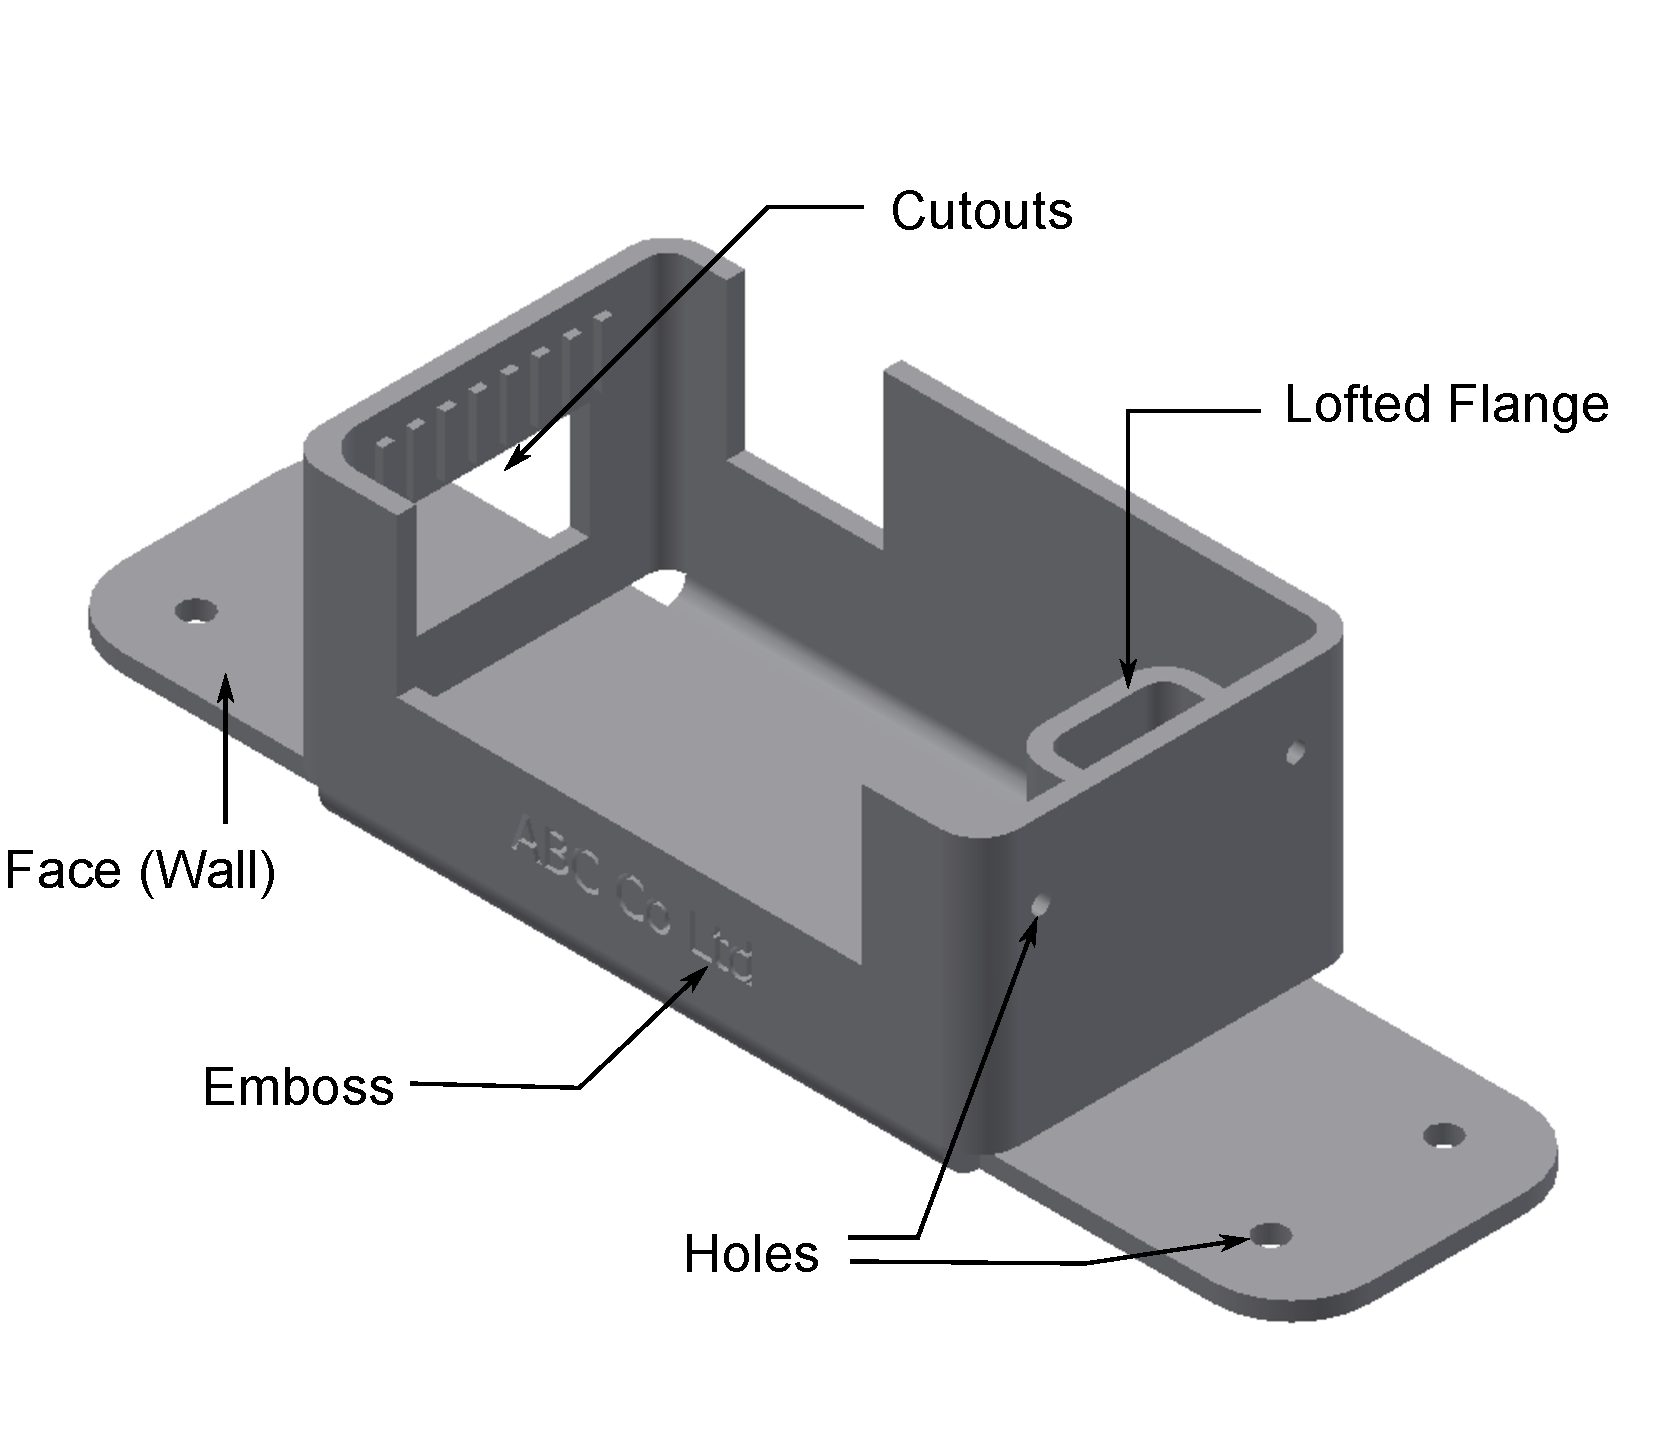
\includegraphics[width=\linewidth,valign=t]{../Common/images/SheetMetal_Medium_Enclosure_OriginalPart_2}
\captionof{figure}{Input Sheet Metal CAD Model} \label{fig:results:originalenclosurepart1}

Input to \mysystemname~has been modeled using Sheet Metal modeling environment of Autodesk Inventor. Figure~\ref{fig:results:originalenclosurepart1} shows the model and Figure~\ref{fig:results:originalenclosureparttree} shows the corresponding feature tree.

The model has 3 cutouts for components interfacing with outside world, letter embossing, a chute for wires and holes for fixing bolts. Sheet metal features such as Face (Wall), Flange, Hole, Lofted Flange, Emboss, etc. have been used. Dependencies amongst features was minimized by not referencing faces or edges of previously modeled features, but by using reference geometries such as planes, axes, etc. 

\end{minipage}
\quad
\begin{minipage}[c]{0.3\linewidth}
\includegraphics[width=\linewidth,valign=t]{../Common/images/SheetMetal_Medium_Enclosure_OriginalTree}
\captionof{figure}{Feature Tree} \label{fig:results:originalenclosureparttree}
\end{minipage}
\end{minipage}

%%\bigskip

%%
%%%%\bigskip
%%
%%\begin{figure}[!h]
%%\centering     %%% not \center
%%\subfloat[Input Model]{\label{fig:results:originalenclosurepart}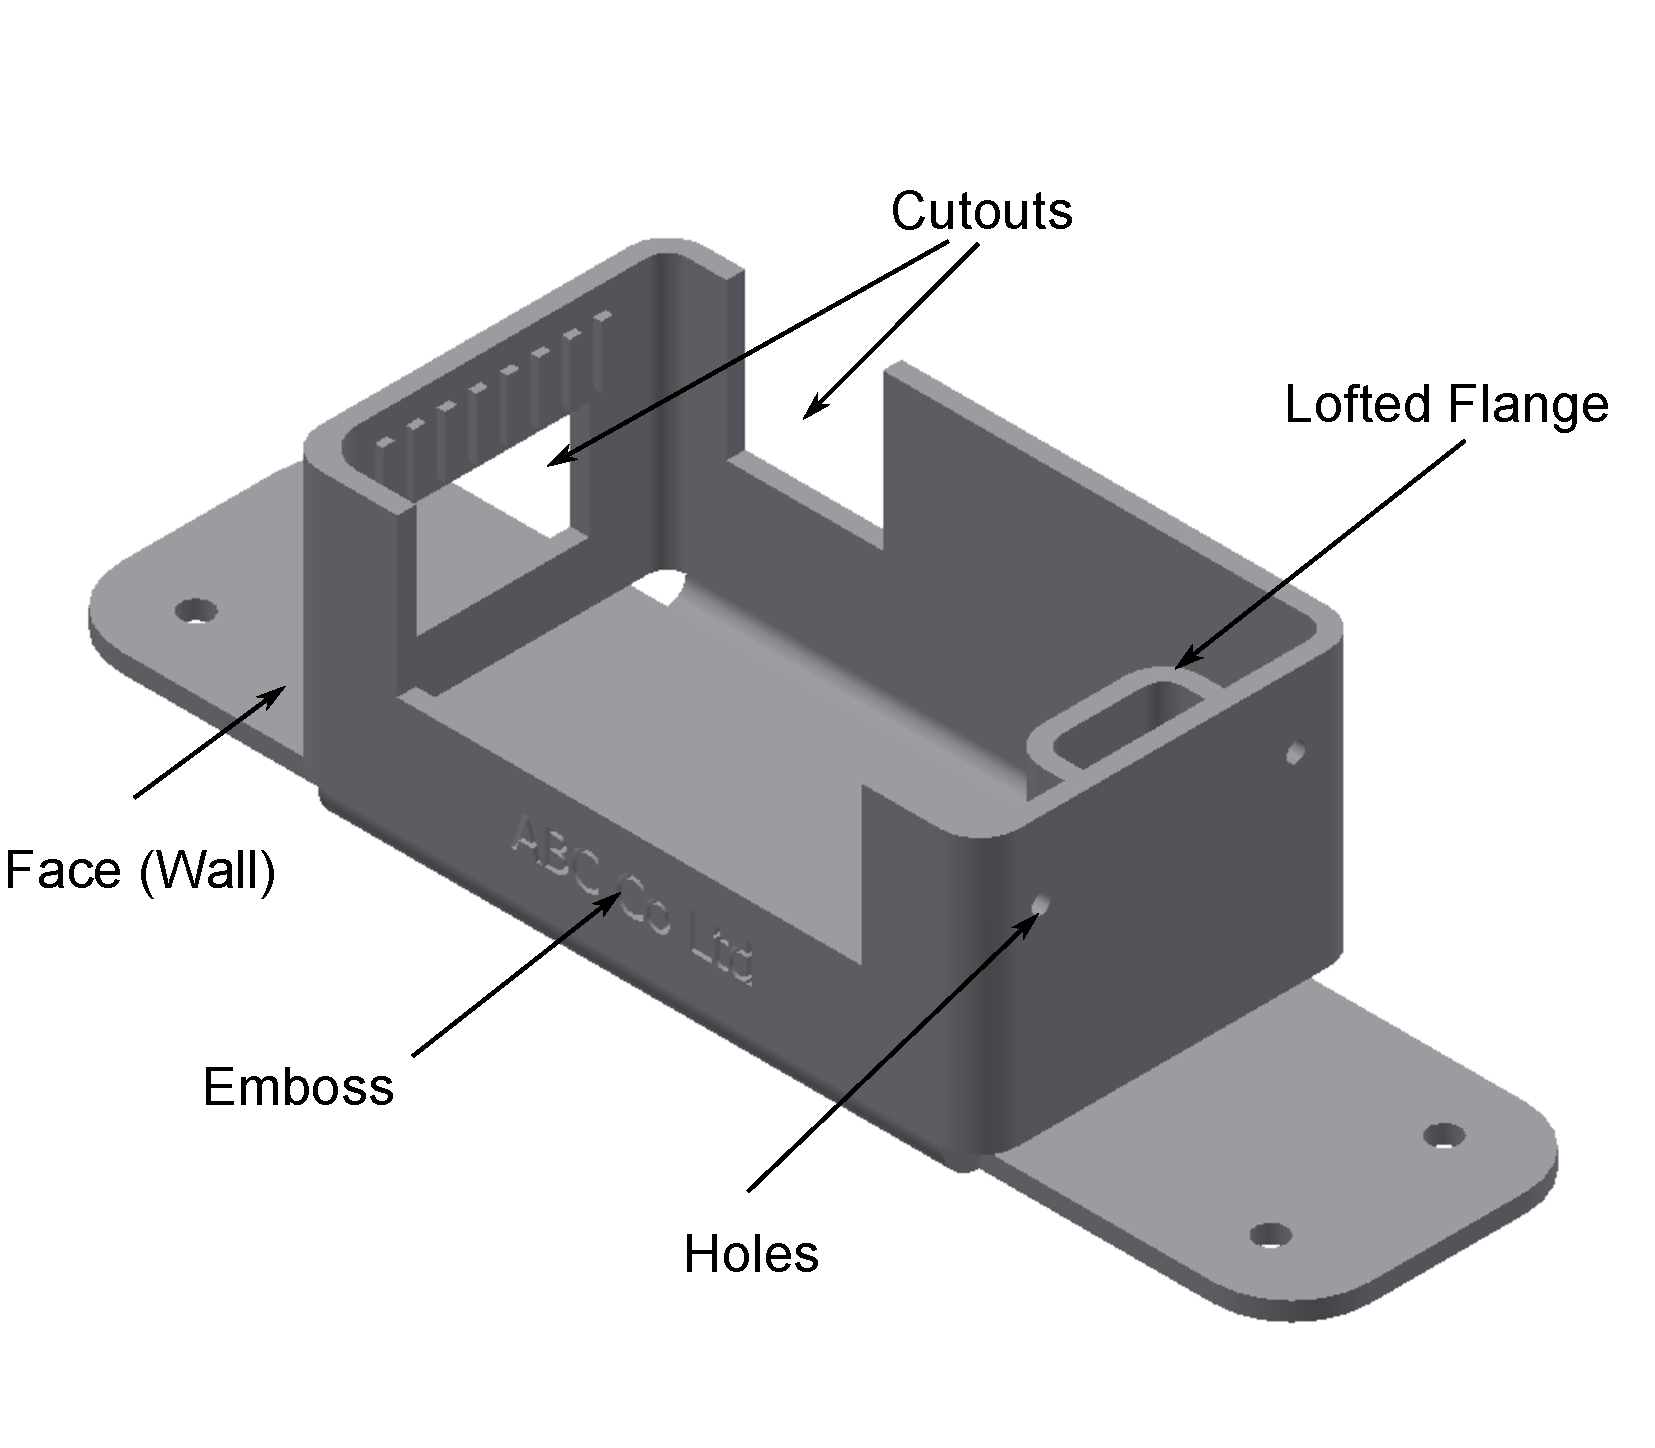
\includegraphics[width=0.55\linewidth,valign=t]{../Common/images/SheetMetal_Medium_Enclosure_OriginalPart_1}} \quad
%%\subfloat[Feature Tree]{\label{fig:results:midsurfbyinventorexnclosure}\includegraphics[width=0.35\linewidth,valign=t]{../Common/images/SheetMetal_Medium_Enclosure_OriginalTree}}
%%\caption{Input CAD model of Enclosure part}
%%\label{fig:results:enlosureinput}
%%\end{figure}
%%
%%
%%%%\bigskip



\subsection{CAD Model Defeaturing}

Defeaturing removes irrelevant features to compute the ``gross shape''. It also caches tool-bodies of relevant negative features to be used for piercing after midsurface computation. Threshold (D) used as a size threshold here is 5\% of the total model size, computed using face-area-summation method.


%%\bigskip

\begin{minipage}{\linewidth}
\begin{minipage}[c]{0.62\linewidth}
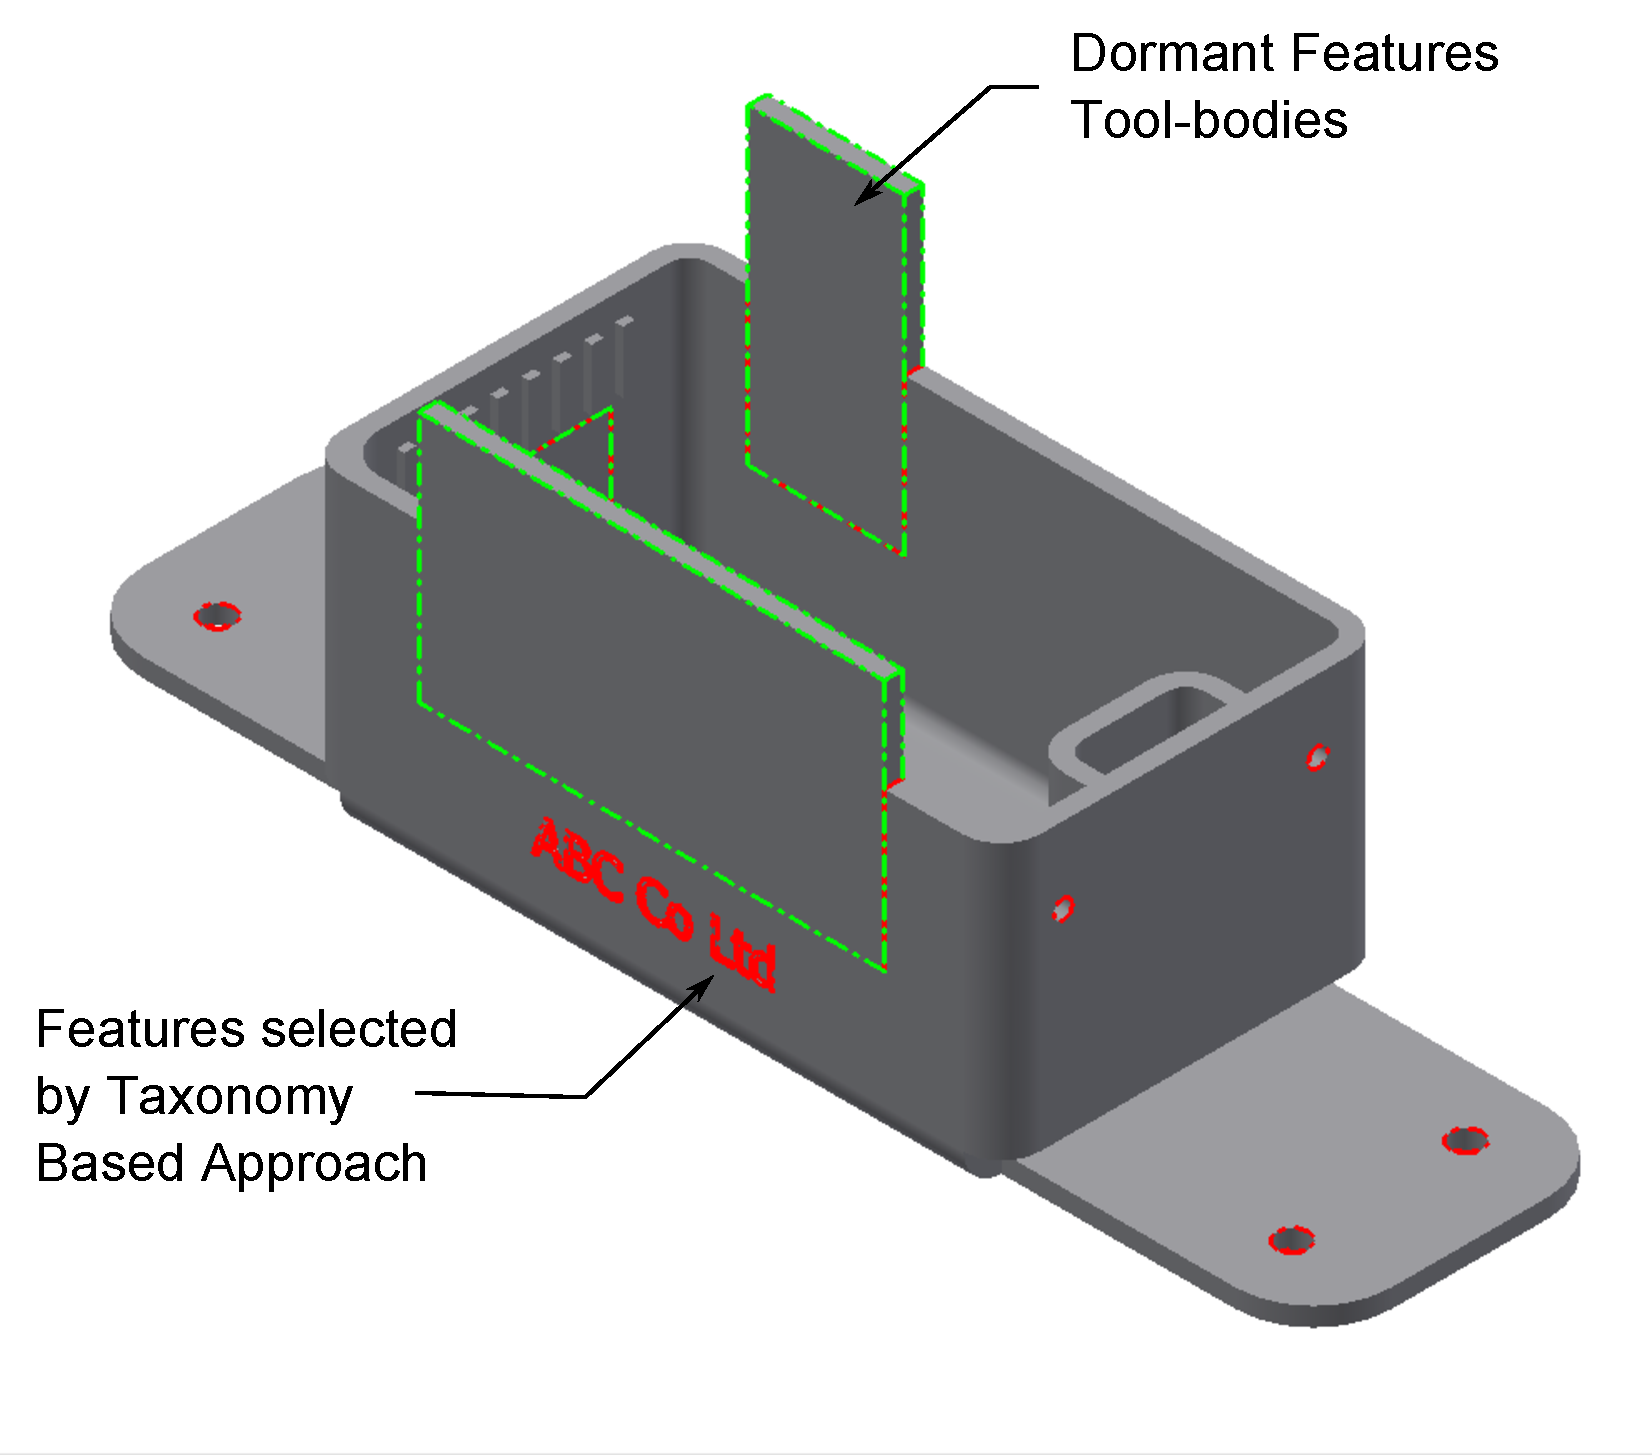
\includegraphics[width=\linewidth,valign=t]{../Common/images/SheetMetal_Medium_Enclosure_PhaseISelections_3}
\captionof{figure}{Selection of Features based on Taxonomy Based and Dormant Features Approach} \label{fig:results:phI}

%%\bigskip
As per defeaturing based on Sheet Metal feature taxonomy rules, elaborated in Section~\ref{sec:defeaturing:phase11}, secondary features chosen for removal are:

\begin{itemize}[noitemsep,topsep=2pt,parsep=2pt,partopsep=2pt]
\item Hole1, Hole2, Hole3, Hole4, Hole5, Hole6
\item Cut4, Cut5, Cut6
\item Emboss2
\end{itemize}

Figure~\ref{fig:results:phI} also shows the identification of dormant features. As elaborated in Section~\ref{sec:defeature:dormant}, relevant negative features are removed after storing their tool-bodies. These tool-bodies, represented by Extrusion9, Extrusion10 and Extrusion11, are shown in Figure~\ref{fig:results:phI} as ``Dormant Features''. Figure~\ref{fig:results:phIsel} shows the same features selected in the feature tree.

\end{minipage}
\quad
\begin{minipage}[c]{0.3\linewidth}
\includegraphics[width=\linewidth,valign=t]{../Common/images/SheetMetal_Medium_Enclosure_PhaseISelectionsTree}
\captionof{figure}{Selected Features for Removal} \label{fig:results:phIsel}
\end{minipage}
\end{minipage}


%%\bigskip

%%
%%%%\bigskip
%%
%%
%%\begin{figure}[!h]
%%\centering     %%% not \center
%%\subfloat[Taxonomy based selections along with Dormant Features]{\label{fig:results:phI}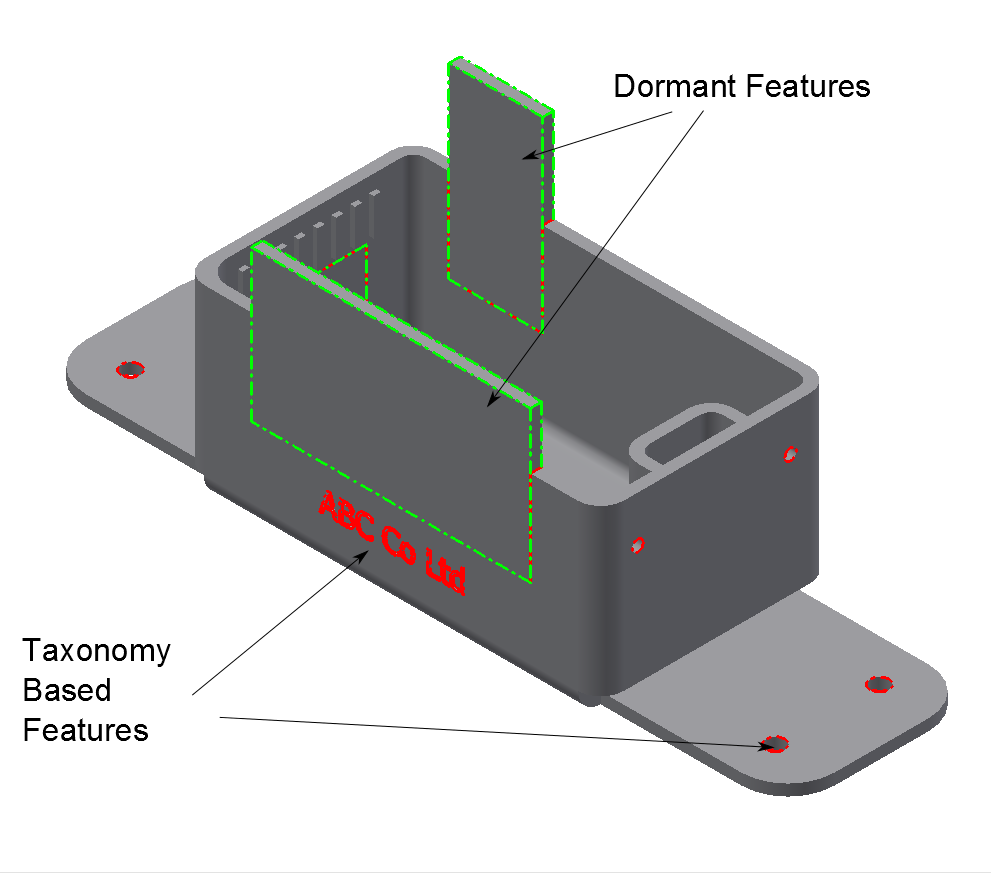
\includegraphics[width=0.62\linewidth,valign=t]{../Common/images/SheetMetal_Medium_Enclosure_PhaseISelections_1}} \quad
%%\subfloat[Selected Features]{\label{fig:results:phIsel}\includegraphics[width=0.17\linewidth,valign=t]{../Common/images/SheetMetal_Medium_Enclosure_PhaseISelectionsTree}}
%%\caption{Defeaturing by Application Context And Dormant features tool bodies}
%%\label{fig:results:enlosurephI}
%%\end{figure}
%%
%%%%\bigskip
%%



\begin{minipage}{\linewidth}
\begin{minipage}[c]{0.62\linewidth}
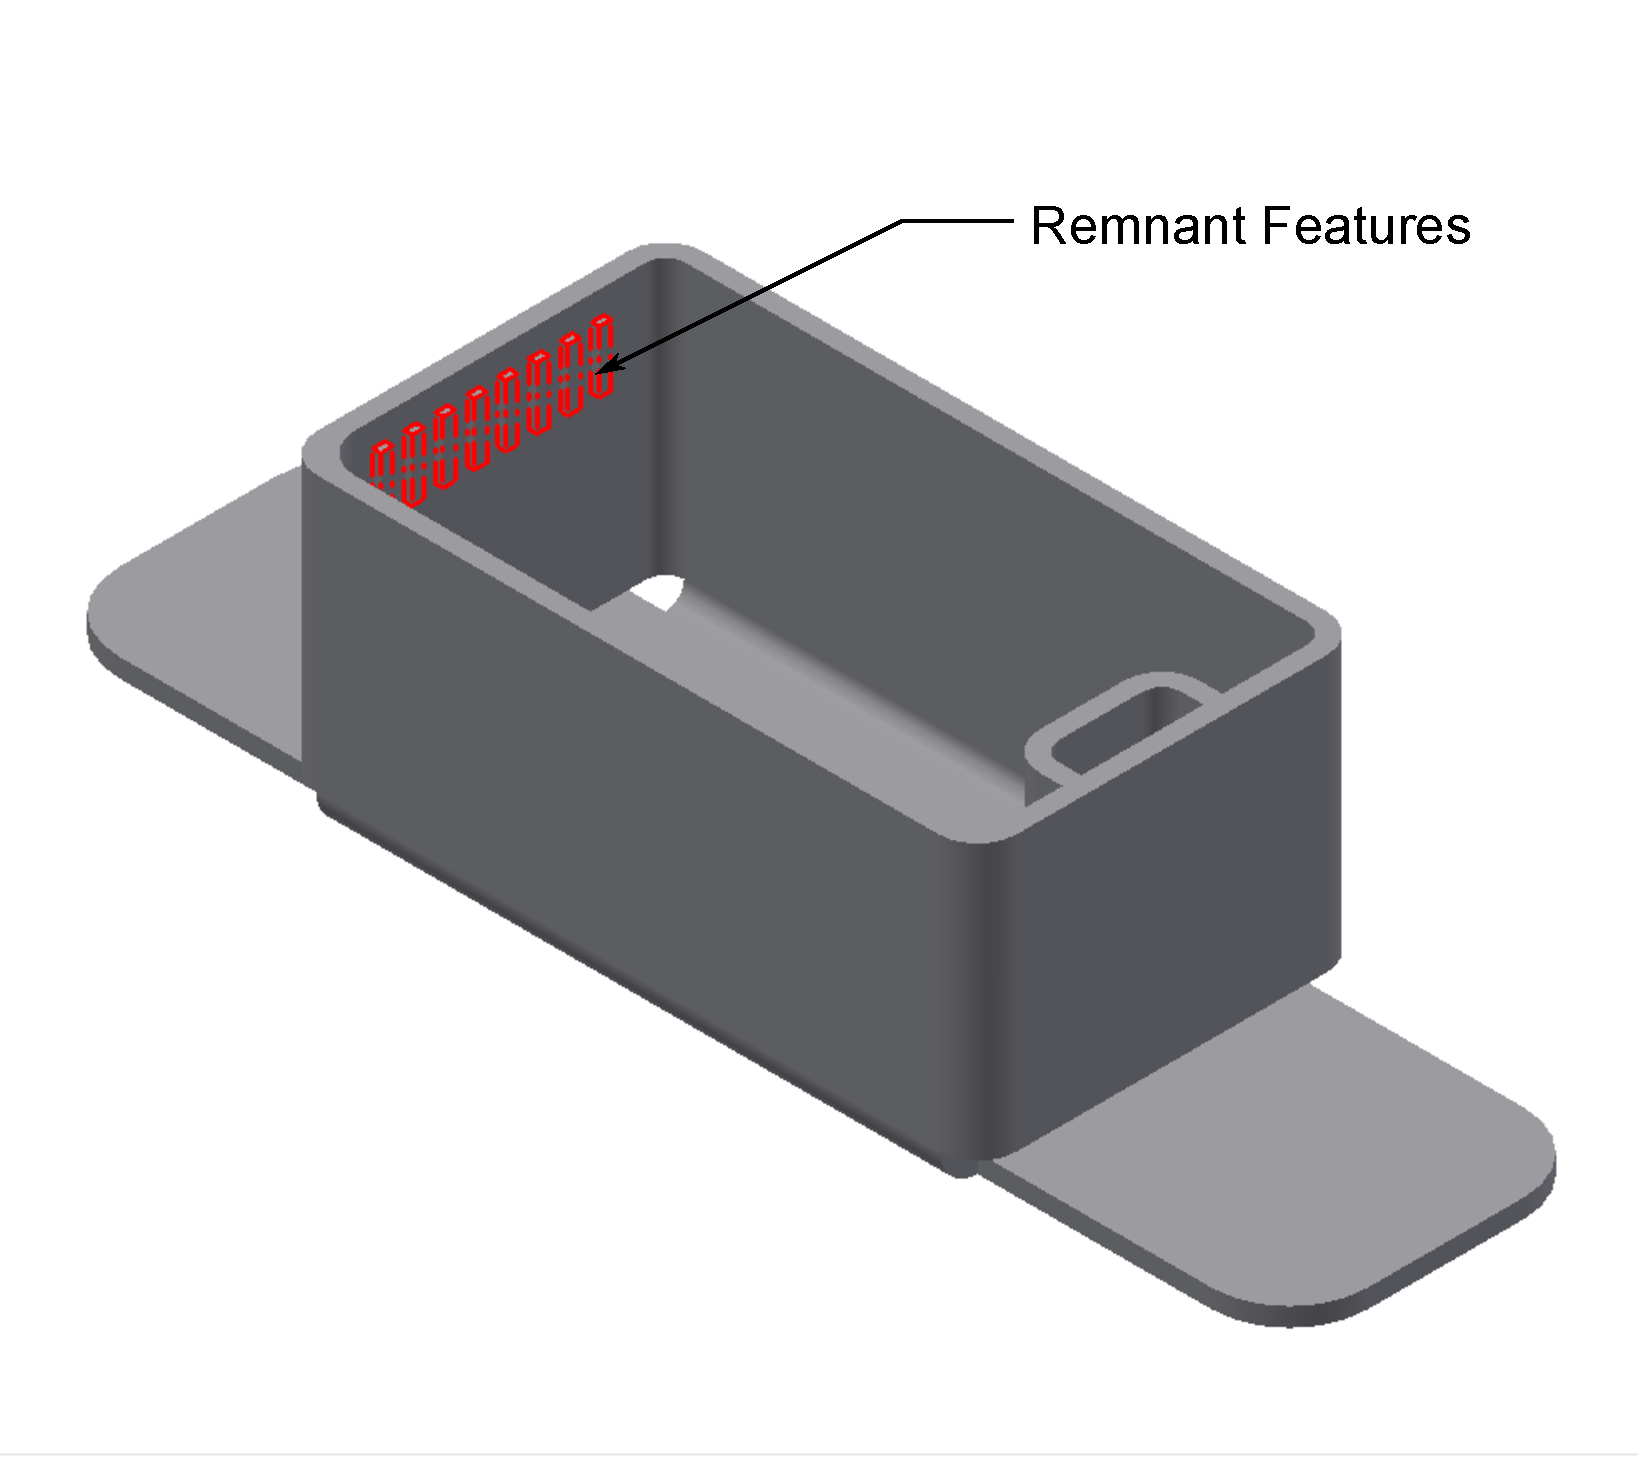
\includegraphics[width=\linewidth,valign=t]{../Common/images/SheetMetal_Medium_Enclosure_PhaseIISelections_3}
\captionof{figure}{Selection of Features based on Remnant Features Approach} \label{fig:results:phII}

%%\bigskip

As per defeaturing based on Remnant feature portions, elaborated in Section~\ref{sec:defeaturing:phase2}, Extrusion1 to 8,  got selected and removed. They were part of array of small protrusions. Their remnant portions were below the threshold size, thus got selected. %Figure~\ref{fig:results:deft} shows the output gross shape of the ``Enclosure'' model.

Figure \ref{fig:results:deft} shows the result of defeaturing process whereas Figure \ref{fig:results:deftfinal} shows the feature tree of the same model. The model has been simplified substantially while retaining the gross shape intent.

\end{minipage}
\quad
\begin{minipage}[c]{0.3\linewidth}
\includegraphics[width=\linewidth,valign=t]{../Common/images/SheetMetal_Medium_Enclosure_PhaseIISelectionsTree}
\captionof{figure}{Selected Features for Removal} \label{fig:results:phIIsel}
\end{minipage}
\end{minipage}


%%\bigskip

%
%%%\bigskip
%
%
%\begin{figure}[!h]
%\centering     %%% not \center
%\subfloat[Remnant based Selections along with Dormant Features]{\label{fig:results:phII}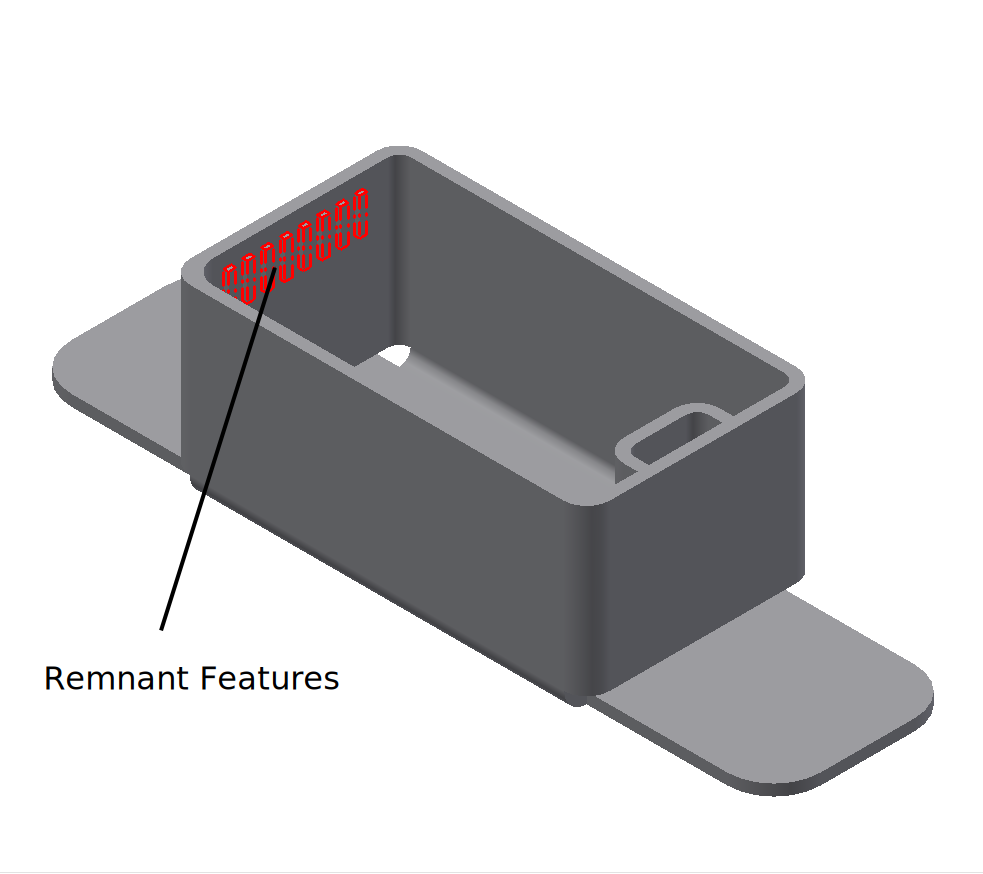
\includegraphics[width=0.62\linewidth,valign=t]{../Common/images/SheetMetal_Medium_Enclosure_PhaseIISelections_1}} \quad
%\subfloat[Selected Features]{\label{fig:results:phIIsel}\includegraphics[width=0.17\linewidth,valign=t]{../Common/images/SheetMetal_Medium_Enclosure_PhaseIISelectionsTree}}
%\caption{Defeaturing by Remnant Features Method}
%\label{fig:results:enlosurephII}
%\end{figure}
%
%
%%%\bigskip

%As per defeaturing based on Remnant feature portions, elaborated in Section~\ref{sec:defeaturing:phase2}, remnant features get selected and removed. Figure~\ref{fig:results:enlosuredeft} shows the gross shape of the ``Enclosure'' model.
%
%Figure \ref{fig:results:deft} shows the result of defeaturing process whereas Figure \ref{fig:results:deftfinal} shows the feature tree of the same model. The model has been simplified substantially while retaining the gross shape intent.

\begin{minipage}{\linewidth}
\begin{minipage}[c]{0.62\linewidth}
\includegraphics[width=\linewidth,valign=t]{../Common/images/SheetMetal_Medium_Enclosure_DefeaturedPart}
\captionof{figure}{Gross Shape after Full Defeaturing} \label{fig:results:deft}

%%\bigskip

Based on Eqn. \ref{eqn:defeaturing:effectiveness}. Defeaturing Effectiveness is computed as follows:

\begin{longtable}[h]{@{} p{0.2\linewidth} p{0.18\linewidth} p{0.3\linewidth} p{0.18\linewidth} @{}}\toprule
\textbf{Entity} & \textbf{Input} & \textbf{After Phase I} & \textbf{Output}\\  \midrule
Faces  & 259 & 104 & 64\\
Features  &  &13 & 8\\
\bottomrule
\label{tbl:fig:defeat}
\end{longtable}

$pR = (1 - \frac{64}{259}) \times 100 = 75.29\%$

\end{minipage}
\quad
\begin{minipage}[c]{0.3\linewidth}
\includegraphics[width=\linewidth,valign=t]{../Common/images/SheetMetal_Medium_Enclosure_DefeaturedTree}
\captionof{figure}{Feature Tree} \label{fig:results:deftfinal}
\end{minipage}
\end{minipage}

%%\bigskip


%%
%%%%\bigskip
%%
%%
%%\begin{figure}[!h]
%%\centering     %%% not \center
%%\subfloat[Gross Shape]{\label{fig:results:deft}\includegraphics[width=0.62\linewidth,valign=t]{../Common/images/SheetMetal_Medium_Enclosure_DefeaturedPart}} \quad
%%\subfloat[Feature Tree]{\label{fig:results:deftfinal}\includegraphics[width=0.17\linewidth,valign=t]{../Common/images/SheetMetal_Medium_Enclosure_DefeaturedTree}}
%%\caption{Gross Shape}
%%\label{fig:results:enlosuredeft}
%%\end{figure}
%%
%%%%\bigskip
%%

%Effectiveness with 5\% threshold, based on the criterion defined by Eqn. \ref{eqn:defeaturing:effectiveness} is:
%
%\begin{minipage}[c]{0.6\linewidth}
%\begin{longtable}[h]{@{} p{0.22\linewidth} p{0.18\linewidth} p{0.21\linewidth} p{0.2\linewidth} @{}}\toprule
%\textbf{Qty} & \textbf{Input} & \textbf{Phase I} & \textbf{Output}\\  \midrule
%Faces  & 259 & 104 & 64\\
%Suppressed  &  &13 & 8\\
%\bottomrule
%\end{longtable}
%\end{minipage}
%\begin{minipage}[c]{0.38\linewidth}
%$pR = (1 - \frac{64}{259}) \times 100 = 75.29\%$
%\end{minipage}
%
%
%Even after huge reduction in the number of faces (75\%), the overall shape of the enclosure is retained fine. This defeatured model is sent to the next module, i.e. Generalization.

\def\myfigenlosuredefeaturecolumnwidth{0.95}
\def\myfigenlosuredefeatureTreecolumnwidth{0.75}
%%\begin{longtable}[h]{@{} p{0.18\linewidth}  p{0.38\linewidth} p{0.1\linewidth} p{0.2\linewidth}@{}}
%%\toprule
%% & Model & Tree & Explanation \\
%% \midrule
%% 
%%Original/Input &
%%\raisebox{-0.8\height}{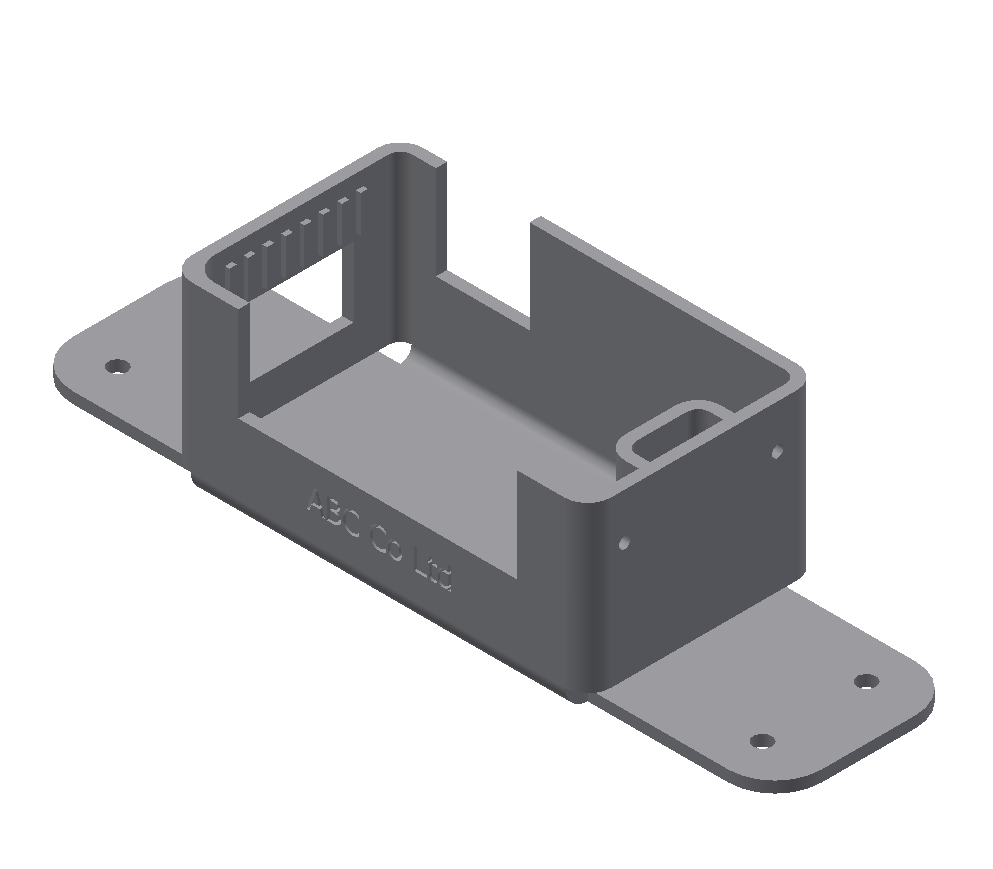
\includegraphics[width=\myfigenlosuredefeaturecolumnwidth\linewidth]{..//Common/images/SheetMetal_Medium_Enclosure_OriginalPart}} &
%%\raisebox{-0.8\height}{\includegraphics[width=\myfigenlosuredefeatureTreecolumnwidth\linewidth]{..//Common/images/SheetMetal_Medium_Enclosure_OriginalTree}} &
%%
%%The model has 3 cutouts for components interfacing with outside world, letter emobssing, a chute for wires and holes for fixing bolts.\\
%%
%%Phase I Selections &
%%\raisebox{-0.8\height}{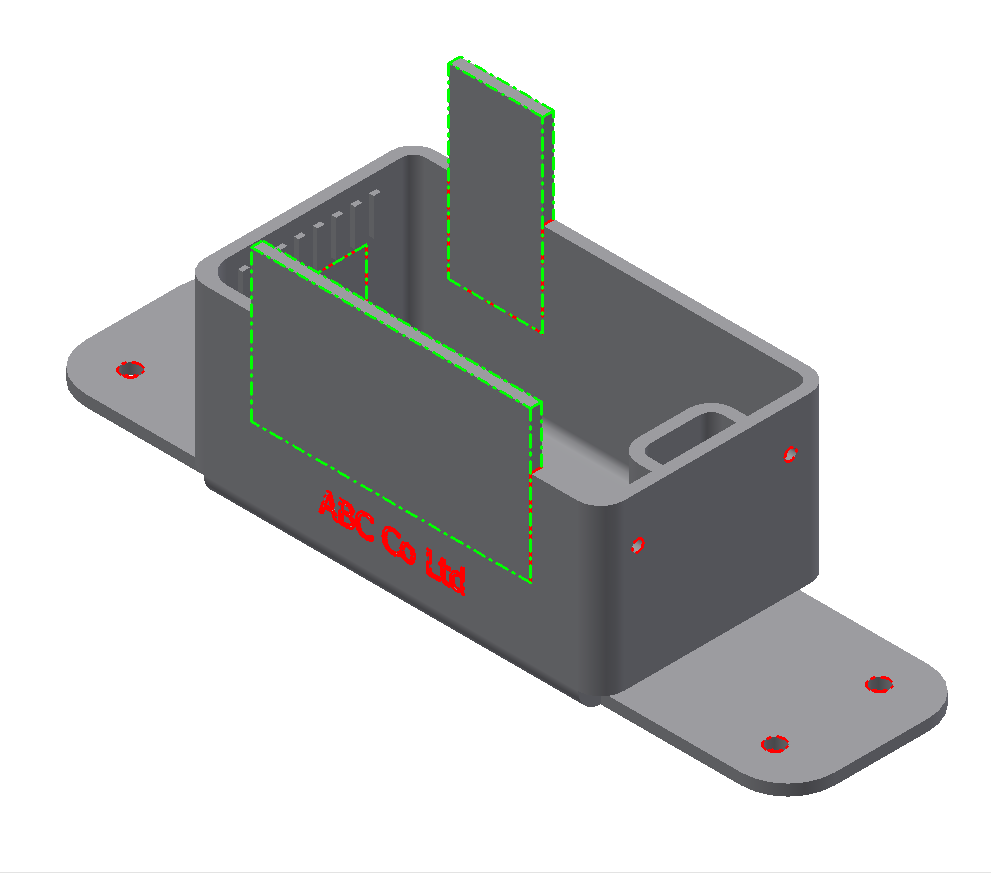
\includegraphics[width=\myfigenlosuredefeaturecolumnwidth\linewidth]{..//Common/images/SheetMetal_Medium_Enclosure_PhaseISelections}} &
%%\raisebox{-0.8\height}{\includegraphics[width=\myfigenlosuredefeatureTreecolumnwidth\linewidth]{..//Common/images/SheetMetal_Medium_Enclosure_PhaseISelectionsTree}} &
%%
%%Small holes, emobssing is chosen based on Sheet Metal feature taxonomy rules (shown red). The green selections are the dormant feature bodies cached.\\
%%
%%Phase II  Selections&
%%\raisebox{-0.8\height}{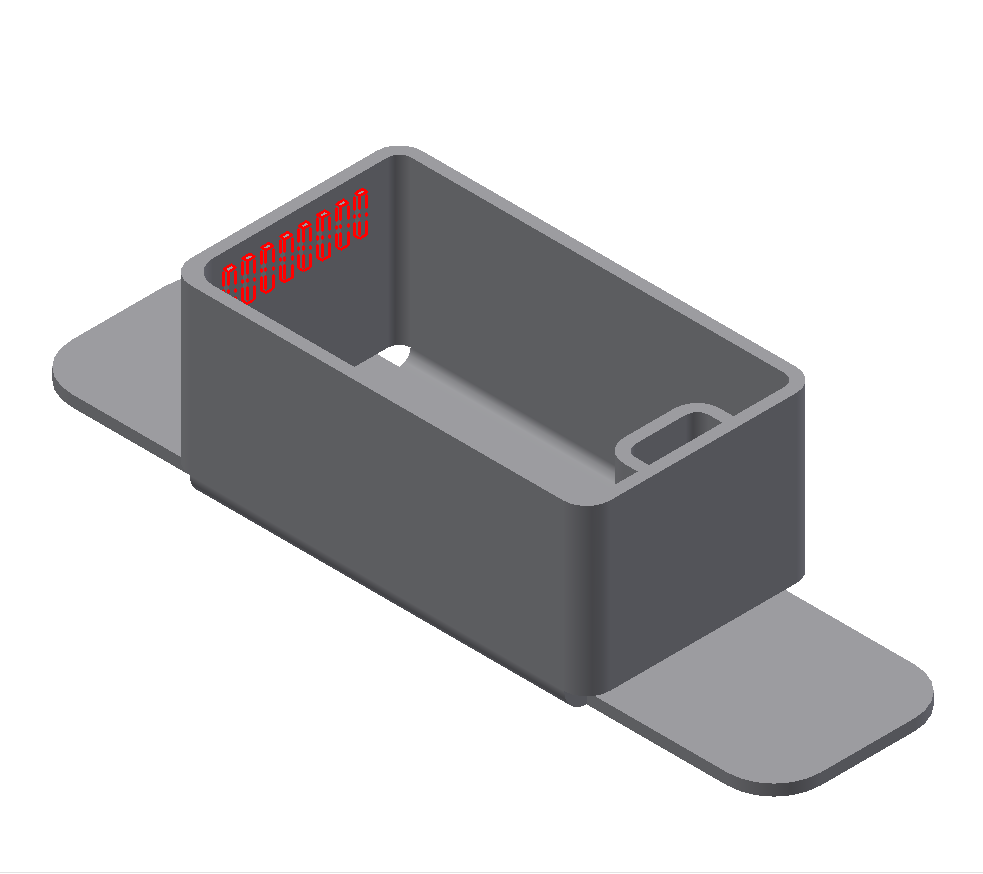
\includegraphics[width=\myfigenlosuredefeaturecolumnwidth\linewidth]{..//Common/images/SheetMetal_Medium_Enclosure_PhaseIISelections}} &
%%\raisebox{-0.8\height}{\includegraphics[width=\myfigenlosuredefeatureTreecolumnwidth\linewidth]{..//Common/images/SheetMetal_Medium_Enclosure_PhaseIISelectionsTree}} &
%%
%%Remnant features got selected in the second phase. \\
%%
%%Defeatured&
%%\raisebox{-0.8\height}{\includegraphics[width=\myfigenlosuredefeaturecolumnwidth\linewidth]{..//Common/images/SheetMetal_Medium_Enclosure_DefeaturedPart}} &
%%\raisebox{-0.8\height}{\includegraphics[width=\myfigenlosuredefeatureTreecolumnwidth\linewidth]{..//Common/images/SheetMetal_Medium_Enclosure_DefeaturedTree}} &
%%
%%Most of the unnecessary features are removed and now it retains all the necessary features adequately ``representing''  the gross shape. \\
%%
%%\bottomrule
%%\end{longtable}

%Based on Eqn. \ref{eqn:defeaturing:effectiveness}. Defeaturing Effectiveness is computed as follows:

%
%%%\bigskip
%
%
%\begin{minipage}[c]{0.6\linewidth}
%\begin{longtable}[h]{@{} p{0.25\linewidth} p{0.18\linewidth} p{0.21\linewidth} p{0.2\linewidth} @{}}\toprule
%\textbf{Qty} & \textbf{Input} & \textbf{Phase I} & \textbf{Output}\\  \midrule
%Faces  & 259 & 104 & 64\\
%Features left  &  &13 & 8\\
%\bottomrule
%\end{longtable}
%\end{minipage}
%\begin{minipage}[c]{0.38\linewidth}
%$pR = (1 - \frac{64}{259}) \times 100 = 75.29\%$
%\end{minipage}
%

%%\bigskip

The Table shows number of faces in the CAD model, at the Input stage, then after application context specific defeaturing (called ``Phase I'') and then at the final stage (called ``Output''). So, overall, the number of faces have reduced from 259 in the input to 64 in the output model. The number of features left after Phase I were 13 whereas 8 were remaining at the end. It can be clearly seen that even after 75\% reduction in number of faces the gross shape of the enclosure retains the overall shape and design intent.

\subsection{CAD Model Generalization}

The purpose of this module is to transform remaining sheet metal features into $\mathcal{ABLE}$ features.

%%\bigskip

\begin{figure}[!h]
\centering     %%% not \center
\subfloat[CAD Feature Tree]{\label{fig:results:midsurfbyinventorexnclosure}\includegraphics[width=0.32\linewidth,valign=t]{../Common/images/SheetMetal_Medium_Enclosure_pre_abel_tree}}\quad
\subfloat[$\mathcal{ABLE}$ Feature tree]{\label{fig:results:able}\includegraphics[width=0.32\linewidth,valign=t]{../Common/images/SheetMetal_Medium_Enclosure_abel_tree}}
\caption{Transformation of CAD Model to Generalized Features}\label{fig:results:enlosurepreable}
\end{figure}

Table~\ref{tbl:results:cadablemap} shows map of Sheet Metal features to their corresponding $\mathcal{ABLE}$ such as Extrude, Sweep, etc. as per approach detailed in Section~\ref{sec:abstraction:sheetmetalfeaturesable}.
%%\bigskip

\begin{table}[!h]
\centering
\caption{Case I: CAD to $\mathcal{ABLE}$ Feature Mapping}
\label{tbl:results:cadablemap}
\begin{tabular}[h]{@{} p{0.21\linewidth} p{0.21\linewidth} @{}}
\toprule
{\bf CAD Feature } & {$\mathcal{ABLE}$ Feature}\\ \midrule
Face3 & Extrusion12\\
Flange1 & Sweep1\\
Flange2 & Sweep2 \\
Face4 & Extrusion13\\
Face5 & Extrusion15\\
Flange4 & Sweep3\\
Flange5 & Sweep4\\
Face8 & Extrusion15\\
Face9 & Extrusion16\\
LoftedFlange1 & Extrusion17\\
\bottomrule
\end{tabular}

\end{table}



 Figure~\ref{fig:results:originalenclosurepart} shows the input model having sheet metal features such as Face-Wall, Flange, Lofted Flange, etc. Figure~\ref{fig:results:preble} shows the transformed feature tree. Algorithms for transforming each of these features are listed in Table~\ref{tbl:abstraction:sheetmetalfeaturesable}.

%%\bigskip

\begin{figure}[!h]
\centering     %%% not \center
\subfloat[Input CAD Model]{\label{fig:results:originalenclosurepart}\includegraphics[width=0.43\linewidth,valign=t]{../Common/images/SheetMetal_Medium_Enclosure_pre_abel_part}} \quad
\subfloat[Transformed $\mathcal{ABLE}$ Model]{\label{fig:results:preble}\includegraphics[width=0.43\linewidth,valign=t]{../Common/images/SheetMetal_Medium_Enclosure_abel_part}} \quad
\caption{Transformation of CAD Model to $\mathcal{ABLE}$ Model}
\label{fig:results:enlosureable}
\end{figure}


%%\bigskip


Thus, after transforming all the sheet metal features in the input model to their $\mathcal{ABLE}$ features, the output $\mathcal{ABLE}$ model retains the overall shape and design intent.

%\def\myfigenlosureabelcolumnwidth{0.98}
%\begin{longtable}[h]{@{} p{0.1\linewidth}  p{0.38\linewidth} p{0.15\linewidth} p{0.2\linewidth}@{}}
%\toprule
% & Model & Tree & Explanation \\
% \midrule
%
%Defeatured Input &
%\raisebox{-0.8\height}{\includegraphics[width=\myfigenlosuredefeaturecolumnwidth\linewidth]{..//Common/images/SheetMetal_Medium_Enclosure_pre_abel_part}} &
%\raisebox{-0.8\height}{\includegraphics[width=\myfigenlosureabelcolumnwidth\linewidth]{..//Common/images/SheetMetal_Medium_Enclosure_pre_abel_tree}} &
%
%The model has Sheet metal features such as FACE, Flange, Lofted Flange etc. ({\footnotesize Limitations in implementation of certain features are corrected manually})\\
%
%Generalized Output &
%\raisebox{-0.8\height}{\includegraphics[width=\myfigenlosuredefeaturecolumnwidth\linewidth]{..//Common/images/SheetMetal_Medium_Enclosure_abel_part}} &
%\raisebox{-0.8\height}{\includegraphics[width=\myfigenlosureabelcolumnwidth\linewidth]{..//Common/images/SheetMetal_Medium_Enclosure_abel_tree}} &
%
%All Sheet Metal features are generalized to basic primitive features such as Extrude, Sweep etc.\\
%
%\bottomrule
%\end{longtable}

\subsection{CAD Model Decomposition}

In the present research work the $\mathcal{ABLE}$ model is appropriately decomposed manually to create solid and interface cells. As elaborated in Section~\ref{sec:fbcd:proposal}, the decomposition is done in two steps viz. Feature partitioning and convex partitioning.  In feature partitioning ``Unite'' booleans are set to ``New Body'' type thereby separating the tool bodies of features. Then feature volumes are split at the concave edges, by Convex Partitioning. Figure~\ref{fig:results:decompoutputmodel} shows the decomposed model and Figure~\ref{fig:results:decompoutputtree} shows the feature tree.

%\begin{figure}[!h]
%\centering     %%% not \center
%\subfloat[Input $\mathcal{ABLE}$  Model]{\label{fig:results:decompinput}\includegraphics[width=0.62\linewidth,valign=t]{../Common/images/SheetMetal_Medium_Enclosure_pre_abel_part}} \quad
%\subfloat[Feature Tree]{\label{fig:results:decompinouttree}\includegraphics[width=0.25\linewidth,valign=t]{../Common/images/SheetMetal_Medium_Enclosure_abel_tree}}
%\caption{Input $\mathcal{ABLE}$  Model}
%\label{fig:results:decompinput}
%\end{figure}

%Feature partitioning is done for separating features' tool bodies. The Concave Edge Partitioning techniques is used to form cells.


%%\bigskip

\begin{figure}[!h]
\centering     %%% not \center
\subfloat[Cells with $\mathcal{ABLE}$ owner features]{\label{fig:results:decompoutputmodel}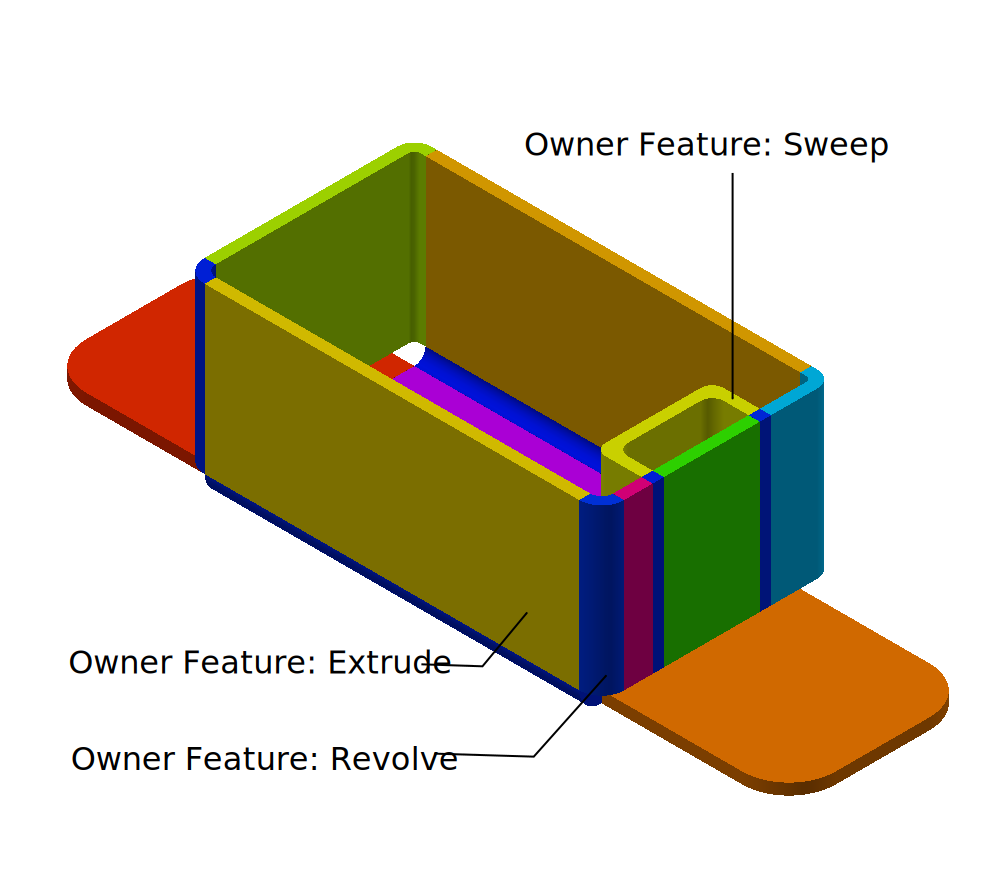
\includegraphics[width=0.6\linewidth,valign=t]{../Common/images/SheetMetal_Medium_Enclosure_decomp_part_2}} \quad
\subfloat[Feature Tree After Decomposition]{\label{fig:results:decompoutputtree}\includegraphics[width=0.3\linewidth,valign=t]{../Common/images/SheetMetal_Medium_Enclosure_decomp_tree}}
\caption{Cellular Decomposition of the Gross Shape}
\label{fig:results:decompoutput}
\end{figure}


%%\bigskip

Thus, the $\mathcal{ABLE}$ model is now transformed into a collection of cells with their respective owner features. 


\todo{Review comment: Clearly show scells and icells. [THIS MODEL HAS NO ICELLS, SO NOT SHOWN ANY]}

%Decomposition is a manual process. As mentioned in Section \ref{sec:midsurfcelljoin:decomposition}, quite a few algorithms are readily available and thus are not presented here as they are not contribution f this work. Due to lack of availability of their source they could not be integrated here. So the decomposition is done manually. Given generalized model, it is decomposed at feature level as well as at convex edges to form cells.% The process followed is:
%\begin{itemize}[noitemsep,topsep=2pt,parsep=2pt,partopsep=2pt]
%\item \textbf{Feature partitioning}: Internal as well as external booleans  are changed to the ``New Body'' type, so that the tool-body volumes get separated. The volumes may still overlap with each other.
%\item \textbf{Concave edge partitioning (CEP)}: Overlapping volumes are split at concave edges. Faces at these edges are extended and used as partitions to split. In this work, extensions are not done infinitely (or covering the part's bounding box) but within the influence zone decided by two interacting features.
%\end{itemize}

%%\def\myfigenlosureabelcolumnwidth{0.98}
%%\begin{longtable}[h]{@{} p{0.1\linewidth}  p{0.38\linewidth} p{0.15\linewidth} p{0.2\linewidth}@{}}
%%\toprule
%% & Model & Tree & Explanation \\
%% \midrule
%%
%%Generalized Input &
%%\raisebox{-0.8\height}{\includegraphics[width=\myfigenlosuredefeaturecolumnwidth\linewidth]{..//Common/images/SheetMetal_Medium_Enclosure_abel_part}} &
%%\raisebox{-0.8\height}{\includegraphics[width=\myfigenlosureabelcolumnwidth\linewidth]{..//Common/images/SheetMetal_Medium_Enclosure_abel_tree}} &
%%
%%Internal booleans of Primitive features are set to ``New'' thus separating their tool bodies. Then partitioning at convex edges is done.\\
%%
%%Decomposed Output &
%%\raisebox{-0.8\height}{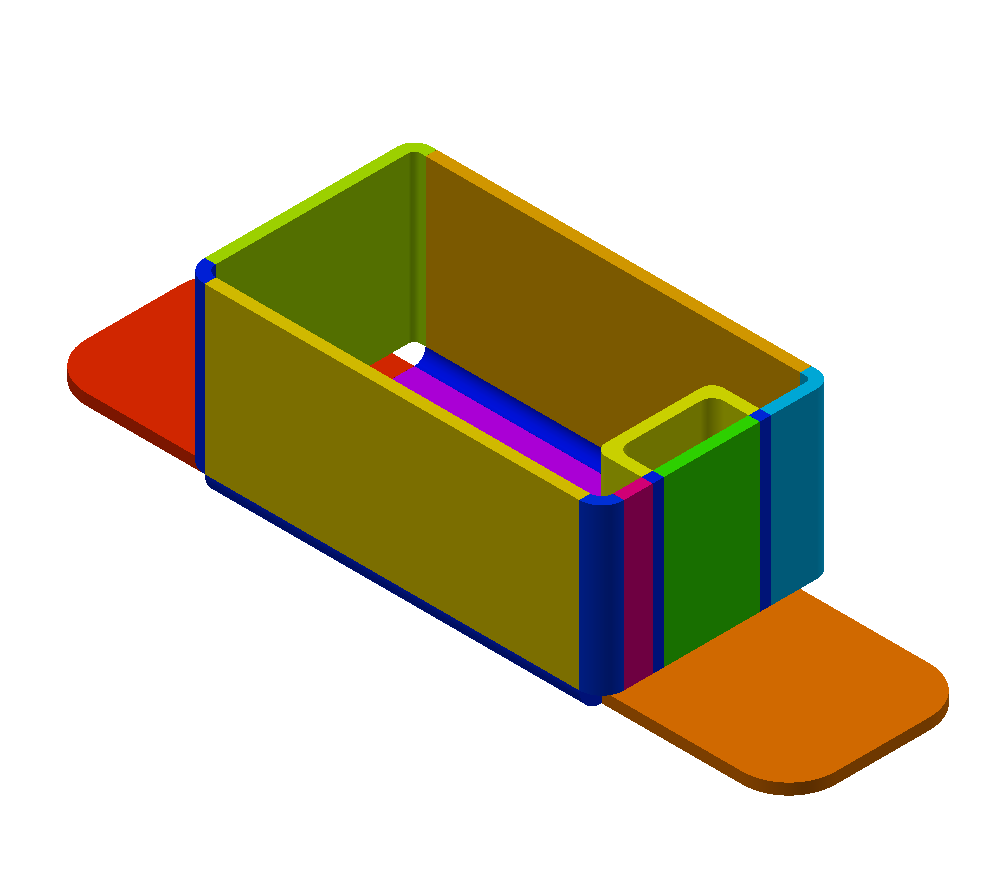
\includegraphics[width=\myfigenlosuredefeaturecolumnwidth\linewidth]{..//Common/images/SheetMetal_Medium_Enclosure_decomp_part}} &
%%\raisebox{-0.8\height}{\includegraphics[width=\myfigenlosureabelcolumnwidth\linewidth]{..//Common/images/SheetMetal_Medium_Enclosure_decomp_tree}} &
%%
%%List of cells with a $\mathcal{ABLE}$ owner feature assigned.\\
%%
%%\bottomrule
%%\end{longtable}


\subsection{Midsurface Generation}

\todo{Review comment: Need to mention purpose of decomposition.[DONE]}
With decomposition, the complex problem of computing midsurface of a model is reduced to a set of more manageable and deterministic sub-problems, i.e. cell-wise midsurface computation. The decomposed model has 14 $sCell$s and 2 $iCell$s.

In the first step, all $sCell$s compute their own midsurface patches. Figure~\ref{fig:results:exscell1} shows an example $sCell$. Its sketch-profile is extracted, and facet-ed as shown in Figure~\ref{fig:results:exprofile1}. Polygon is decomposed as depicted in Figure~\ref{fig:results:exdecomp1} and  Figure~\ref{fig:results:exmidcurve1} shows the output midcurve, which is extruded to compute the midsurface patch.


%%\bigskip


\begin{figure}[!h]
\centering     %%% not \center
\subfloat[Example Solid Cell]{\label{fig:results:exscell1}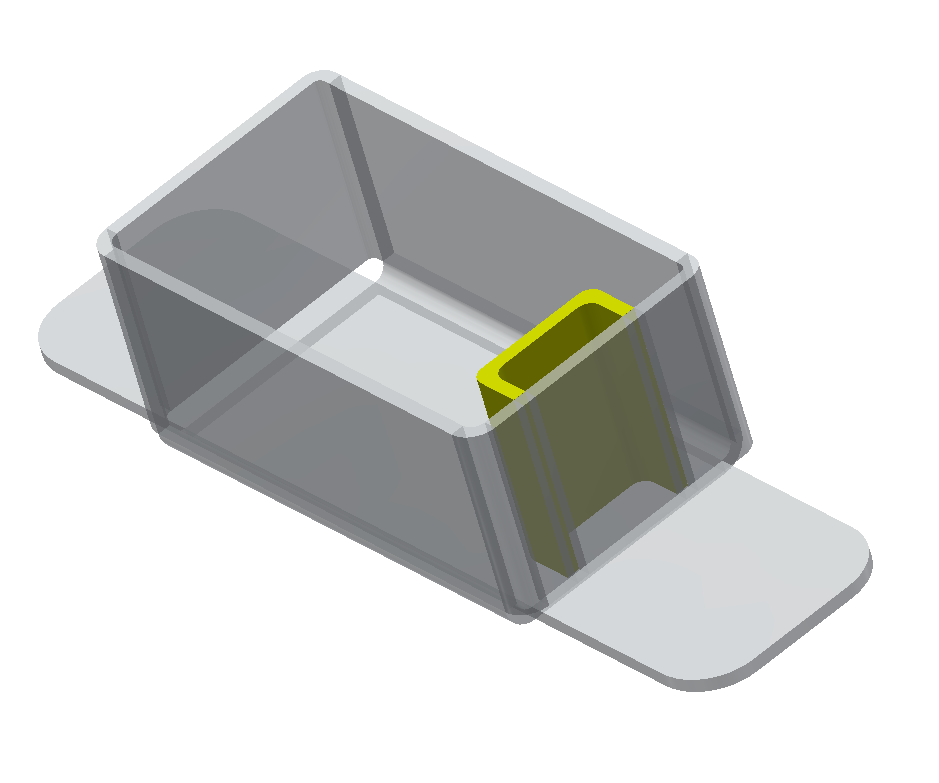
\includegraphics[width=0.34\linewidth,valign=t]{../Common/images/UsCellinModel}}\hfill
\subfloat[Profile Polygon]{\label{fig:results:exprofile1}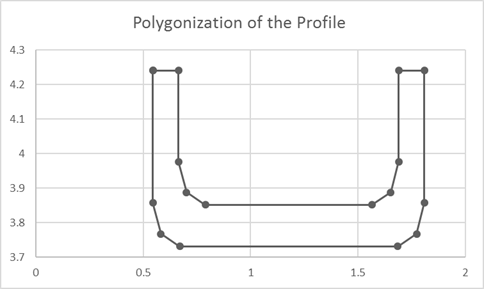
\includegraphics[width=0.46\linewidth,valign=t]{../Common/images/UsCellPolygon}}\hfill
\subfloat[Polygon Decomposition]{\label{fig:results:exdecomp1}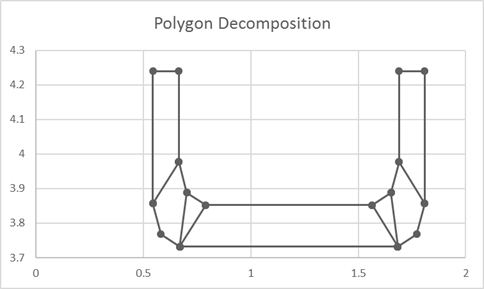
\includegraphics[width=0.46\linewidth,valign=t]{../Common/images/UsCellDecomp}}\hfill
\subfloat[Resultant Midcurve]{\label{fig:results:exmidcurve1}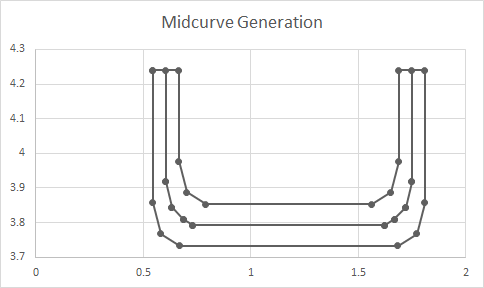
\includegraphics[width=0.46\linewidth,valign=t]{../Common/images/UsCellMidcurve}}
\caption{Midcurve Computation of a Solid Cell}\label{fig:results:midcurvescell1}
\end{figure}



%%\bigskip


\begin{figure}[!h]
\centering     %%% not \center
\subfloat[Midsurface Patches from all Solid Cells]{\label{fig:results:scellspatches}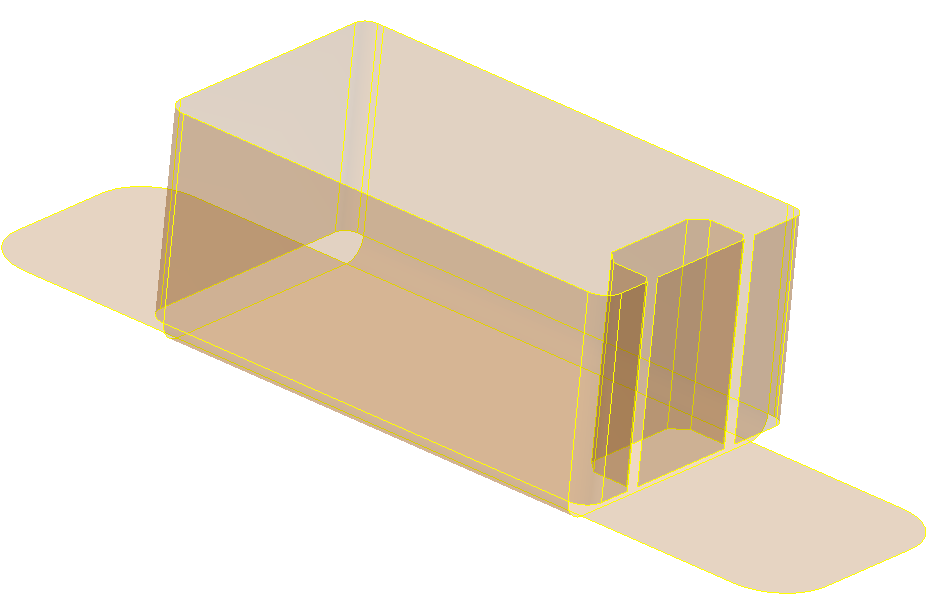
\includegraphics[width=0.46\linewidth,valign=t]{../Common/images/EnclosureOnlysCells}}\hfill
\subfloat[Gaps at Interface Cell Locations]{\label{fig:results:gapsicells}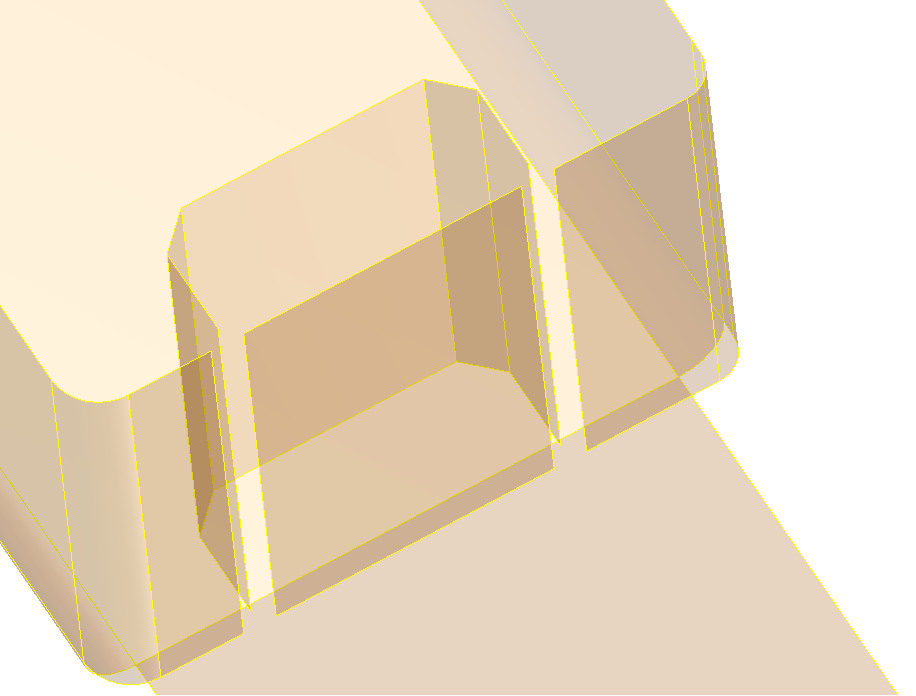
\includegraphics[width=0.38\linewidth,valign=t]{../Common/images/EnclosureOnlysCellsZoom}}
\caption{Midsurface Patches at $sCell$s}\label{fig:results:enlosurescells}
\end{figure}


%%\bigskip


Figure~\ref{fig:results:scellspatches} shows the output of this step.Figure~\ref{fig:results:gapsicells} shows magnified portion where midsurface patches are yet to be joined.

In the next step, midsurface pacthes are joined together at the $iCell$s. %Figure~\ref{fig:results:icellsjoining} shows the process.


\begin{figure}[!h]
\centering     %%% not \center
\subfloat[Interface Cells $f_3$, $f_5$]{\label{fig:results:twojunct}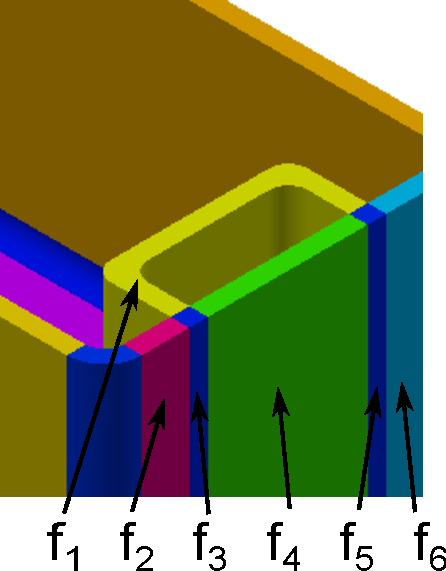
\includegraphics[width=0.25\linewidth,valign=t]{../Common/images/SheetMetal_Medium_Enclosure_decomp_part_small.pdf}} \quad
\subfloat[Connections at Interface Cells]{\label{fig:results:twoicells}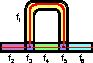
\includegraphics[width=0.48\linewidth,valign=t]{../Common/images/Enclosureicells.pdf}}
\caption{Interface Cells Connecting Midsurface Patches}
\label{fig:results:icellsjoining}
\end{figure}



Figure~\ref{fig:results:icellsjoining} shows working of the midsurface patch joining approach. Figure~\ref{fig:results:twojunct} depicts subset of the model. It shows two interface ($iCell$) cells, attached in two ``T'' type junctions. Cells with owner features $f_3$ and $f_5$ are the $iCell$s, and rest are the $sCell$s. Figure~\ref{fig:results:twoicells} shows, schematically, how extensions are performed with a generic rule specified in Section~\ref{sec:midsurfcelljoin:icell}.


Figure~\ref{fig:results:midsurfcells} shows midsurface patches and their connections resulting into a well connected midsurface. 

\todo{Reviewer comments: Need a very deatied explanantion that how you have computed midsurface. [NOT SURE IF WE NEED TO REPEAT THE SAME INFORMATION. IT IS I GUESS REDUNDANT TO EXPLAIN EACH SCELL AND ICELL WORKING WITH LOTS OF FIGURES HERE]}



%%\bigskip


\begin{figure}[!h]
\centering     %%% not \center
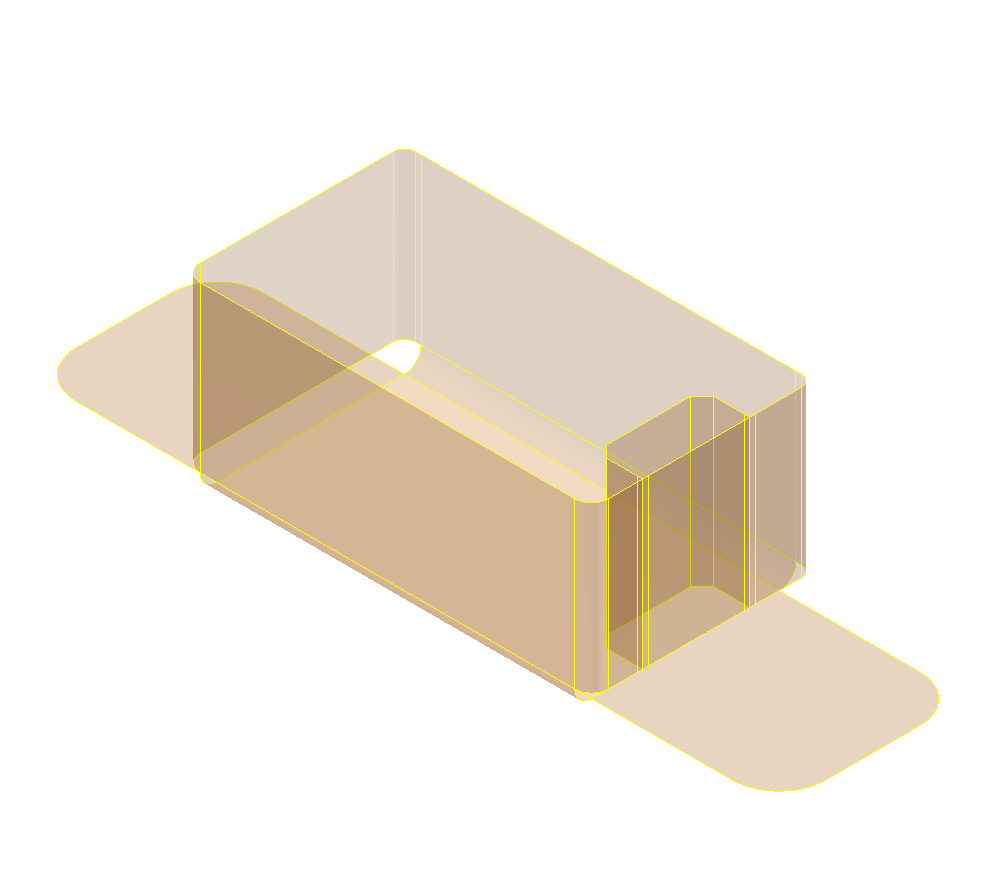
\includegraphics[width=0.62\linewidth,valign=t]{../Common/images/SheetMetal_Medium_Enclosure_midsurf_part}
\caption{Connected Midsurface After Processing of All Solid and Interface Cells}
\label{fig:results:midsurfcells}
\end{figure}


%%\bigskip


As seen in Figure~\ref{fig:results:midsurfcells}, the output is a well-connected midsurface. Use of Cellular topology has removed need of face-pairing approach altogether. It has simplified the problem domain considerably. Thus the midsurface computation has become more generic and agnostic to complexity of the input model.


\subsection{Dormant Feature Re-application}

Midsurface generated at this stage is not final yet. As elaborated in Section \ref{sec:defeaturing:phase11}, during defeaturing, negative features are removed even though they are  relevant. The intent is to make midsurface computation simpler. These temporarily removed features, called Dormant features, are reinstated back on the midsurface here.


%%\bigskip


\begin{figure}[!h]
\centering     %%% not \center
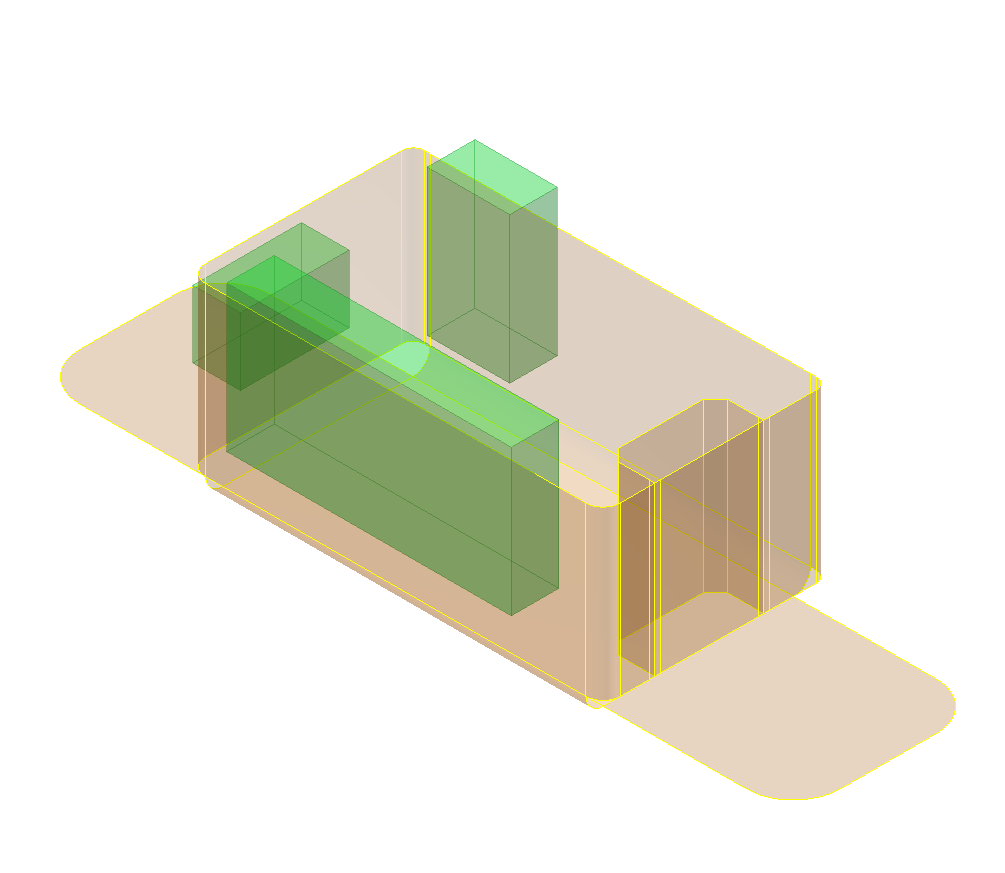
\includegraphics[width=0.62\linewidth,valign=t]{../Common/images/SheetMetal_Medium_Enclosure_dormant_part}
\caption{Re-application of Dormant Feature Tool-bodies on the Connected Midsurface}
\label{fig:results:dormantenclosure}
\end{figure}



%%\bigskip


Cached dormant feature tool bodies are pierced into the midsurface to restore the temporarily-suppressed  negative features. Figure~\ref{fig:results:dormantenclosure} shows the tool-bodies being re-applied on the midsurface, whereas Figure~\ref{fig:results:outputmidsurfenclosure} shows the output final midsurface.



\subsection{Final Output}

%%\bigskip

\begin{figure}[!h]
\centering     %%% not \center
\includegraphics[width=0.62\linewidth,valign=t]{../Common/images/SheetMetal_Medium_Enclosure_final_midsurf_part}
\caption{Output Midsurface computed by \mysystemname}
\label{fig:results:outputmidsurfenclosure}
\end{figure}

%%\bigskip

Figure~\ref{fig:results:outputmidsurfenclosure} shows the final midsurface output computed by \mysystemname.  It has well-connected midsurface, does not have irrelevant features and has maintained the flow of input model shape with fidelity. It is the desired output.

%
%
%\subsection{Benchmarking}

In order to compare the output midsurface, its benchmarking is done against the output by a commercial system. Figure \ref{fig:results:InventorMidsurfwithErrors} shows the midsurface computed by a commercial CAD-CAE system.

\todo{Review comment: Add feature trees. [NOT DONE THAT AS IT WILL CLUTTER HERE. INDIVIDUAL MODULE WISE FEATURE TREES ARE ADDED ANYWAY]}

%\def\myfigenlosurebenchmarkcolumnwidth{0.35} %0.466
%\def\myfigenlosurebenchmarkcolumnwidthaaa{0.55} %0.466

%%\bigskip


\begin{figure}[!h]
\centering     %%% not \center
\includegraphics[width=0.62\linewidth,valign=t]{../Common/images/SheetMetal_Medium_Enclosure_InventorMidsurfwithErrors.pdf}
\caption{Midsurface computed by a Commercial System}
\label{fig:results:InventorMidsurfwithErrors}
\end{figure}

%%\bigskip

%
%\begin{figure}[!h]
%\centering     %%% not \center
%\subfloat[Original Part]{\label{fig:results:originalenclosurepart}\includegraphics[width=0.45\linewidth,valign=t]{../Common/images/SheetMetal_Medium_Enclosure_OriginalPart}} \quad
%\subfloat[Commercial System]{\label{fig:results:InventorMidsurfwithErrors}\includegraphics[width=0.45\linewidth,valign=t]{../Common/images/SheetMetal_Medium_Enclosure_InventorMidsurfwithErrors}}
%\caption{Computation of Midsurface of an Enclosure Model}
%\label{fig:results:enlosurebenchmark}
%\end{figure}
%
%
%%%\bigskip

There are few critical problems in the output midsurface computed by a commercial CAD-CAE system. At two places, the midsurface patches are missing. The lettering (i.e Embossing) has several problems. The Emboss should have been removed altogether.% Analysis of these failures suggests that at two filleted corners, face pairing did not happen properly and thus those midsurface patches were not created, leaving big gaps in the output midsurface. Currently these gaps have to be fixed manually by using ``patch' or `fill' surface modeling operations. %Intent of this case study is to observe \mysystemname's performance compared to the output shown in Figure~\ref{fig:results:InventorMidsurfwithErrors}.

Following are some of the salient conclusions with regard to the test case elaborated above:

\begin{itemize}[noitemsep,topsep=2pt,parsep=2pt,partopsep=2pt]
\item Defeaturing module reduced complexity of the input model substantially (about 75\% reduction in number of faces) and still retained the gross shape.
\item Generalization module reduced variety of sheet metal to a limited set of $\mathcal{ABLE}$ features.
\item Decomposition module reduced the complexity further by dividing the model in to manageable set of cells.
\item Midsurface was computed from the cells using generic rules, compared to some of the existing approaches where case-to-case heuristics has to be applied.
\item Compared to the output by a commercial CAD-CAE system, the midsurface computed by \mysystemname~clearly has a better output.
\end{itemize}
\todo{Review comment: follow the style in the reference thesis. [NOT SURE IF IT IS THE SECTION NUMBERINGS AS `A',`B' ETC]}


Following sections demonstrate efficacy of \mysystemname~using few other real-life sheet metal part models.
%----------------------------------------------------------------------------------------------------------------------------------------------------------------------------------------------------------------

\section{Case Study II}

This case study tests \mysystemname~for computing midsurface of a Stapler model. The household paper stapler has two parts, top and bottom. The bottom part is chosen for benchmarking as its midsurface computed from a commercial CAE system had errors. The intent of this exercise, is to compare it with the output generated by \mysystemname.


\subsection{Input CAD Model}

Stapler CAD model, which is input to \mysystemname~is modeled using Sheet Metal modeling environment of Autodesk Inventor.  Figure~\ref{fig:results:staplerlowermodel} shows the model and Figure~\ref{fig:results:staplerlowermodeltree} shows the corresponding feature tree.


%%\bigskip

\begin{minipage}{\linewidth}
\begin{minipage}[c]{0.62\linewidth}
\includegraphics[width=\linewidth,valign=t]{../Common/images/StaplerLower_1_model.pdf}
\captionof{figure}{Input Sheet Metal CAD Model} \label{fig:results:staplerlowermodel}
Sheet metal features such as Face (Wall), Flange, Hole, Emboss, etc. have been used. Dependencies amongst features was minimized by not referencing faces or edges of previously modeled features, but by using reference geometries such as planes, axes, etc. 
\end{minipage}
\quad
\begin{minipage}[c]{0.3\linewidth}
\includegraphics[width=\linewidth,valign=t]{../Common/images/StaplerLower_1_tree}
\captionof{figure}{Feature Tree} \label{fig:results:staplerlowermodeltree}
\end{minipage}
\end{minipage}


%%\bigskip

%
%%%\bigskip
%
%\begin{figure}[!h]
%\centering     %%% not \center
%\includegraphics[width=0.62\linewidth,valign=t]{../Common/images/StaplerLower_1}
%\caption{Stapler CAD Model}
%\label{fig:results:staplerlowermodel}
%\end{figure}
%


Following subsections show progress of this model through various modules of \mysystemname.

\subsection{CAD Model Defeaturing}

Defeaturing removes irrelevant features to compute the ``gross shape''. It also caches tool-bodies of relevant negative features to be used for piercing after midsurface computation. \deleted{Threshold (D) used as a size threshold here is 5\% of the total part size.}

As per defeaturing based on Sheet Metal feature taxonomy rules, elaborated in Section~\ref{sec:defeaturing:phase11}, secondary features chosen for removal, as seen in Figure~\ref{fig:results:staplerlowerphImodel} and ~\ref{fig:results:staplerlowerphItree}, are:

\begin{itemize}[noitemsep,topsep=2pt,parsep=2pt,partopsep=2pt]
\item CornerRound1, CornerRound5
\item Fillet5, Fillet6
\item Cut1, Cut5
\item Emboss1, Emboss2
\end{itemize}

Figure~\ref{fig:results:staplerlowerphImodel} also shows the identification of dormant features, two holes. As elaborated in Section~\ref{sec:defeature:dormant}, relevant negative features, such as Cutouts in the example shown (features Cut1 and Cut5), are removed after storing their tool-bodies. These Dormant Features' tool-bodies, represented by Extrusion2 and Extrusion3, are shown in Figure~\ref{fig:results:staplerlowerphImodel}. 

%%\bigskip

\begin{minipage}{\linewidth}
\begin{minipage}[c]{0.62\linewidth}
\includegraphics[width=\linewidth,valign=t]{../Common/images/StaplerLower_PhISelections_1_model}
\captionof{figure}{Features Selected for Removal } \label{fig:results:staplerlowerphImodel}

%%\bigskip

The `'Pin Press'' site, as shown in Figure~\ref{fig:results:staplerlowerphImodel} presents peculiar case. This portion is not thin, is not part of oeverll shape, so should be removed. Only due to remnant feature approach this portion was detected and removed. Such removal is not seen in any reviewed approaches.
\end{minipage}
\quad
\begin{minipage}[c]{0.3\linewidth}
\includegraphics[width=\linewidth,valign=t]{../Common/images/StaplerLower_PhISelections_1_tree}
\captionof{figure}{Feature Tree} \label{fig:results:staplerlowerphItree}
\end{minipage}
\end{minipage}

%%\bigskip

%%%\bigskip
%
%\begin{figure}[!h]
%\centering     %%% not \center
%\includegraphics[width=0.62\linewidth,valign=t]{../Common/images/StaplerLower_PhISelections_1.pdf}
%\caption{Selected features for Defeaturing}
%\label{fig:results:staplerlowerphI}
%\end{figure}
%
%%%\bigskip


\begin{minipage}{\linewidth}
\begin{minipage}[c]{0.62\linewidth}
\includegraphics[width=\linewidth,valign=t]{../Common/images/StaplerLower_defeatured_model}
\captionof{figure}{Defeatured Model} \label{fig:results:staplerlowerdefeatmodel}

%%\bigskip

Based on Eqn. \ref{eqn:defeaturing:effectiveness}. Defeaturing Effectiveness is computed as follows:

$pR = (1 - \frac{62}{296}) \times 100 = 79.05\%$
\end{minipage}
\quad
\begin{minipage}[c]{0.3\linewidth}
\includegraphics[width=\linewidth,valign=t]{../Common/images/StaplerLower_defeatured_tree}
\captionof{figure}{Feature Tree} \label{fig:results:staplerlowerdefeattree}
\end{minipage}
\end{minipage}


%%\bigskip

%%%\bigskip
%
%\begin{figure}[!h]
%\centering     %%% not \center
%\includegraphics[width=0.62\linewidth,valign=t]{../Common/images/StaplerLower_defeatured}
%\caption{Gross Shape Stapler}
%\label{fig:results:staplerlowerdefeat}
%\end{figure}
%
%%%\bigskip

The output gross shape is shown in Figure~\ref{fig:results:staplerlowerdefeatmodel}. The overall shape and the design intent is well preserved in the gross shape.

\subsection{CAD Model Generalization}

The purpose of this module is to transform remaining sheet metal features into $\mathcal{ABLE}$ features. Figure~\ref{fig:results:StaplerLowerable} shows feature tree of the input defeatured model as well as the transformed $\mathcal{ABLE}$ features' tree. 

%%\bigskip

\begin{figure}[!h]
\centering     %%% not \center
\subfloat[CAD Feature Tree]{\label{fig:results:midsurfbyinventorStaplerLower}\includegraphics[width=0.32\linewidth,valign=t]{../Common/images/StaplerLower_pre_abel_tree}}\quad
\subfloat[$\mathcal{ABLE}$ Feature tree]{\label{fig:results:StaplerLowerable}\includegraphics[width=0.32\linewidth,valign=t]{../Common/images/StaplerLower_abel_tree}}
\caption{Transformation of CAD Model to Generalized Features}\label{fig:results:StaplerLowerfullable}
\end{figure}


%%\bigskip

Table~\ref{tbl:results:cadablemapstapler} shows how all Sheet Metal features are generalized to their corresponding $\mathcal{ABLE}$ such as Extrude, Sweep, etc. as per approach detailed in Section~\ref{sec:abstraction:sheetmetalfeaturesable}.

%%\bigskip

\begin{table}[!h]
\centering
\caption{Case II: CAD to $\mathcal{ABLE}$ Feature Mapping}
\label{tbl:results:cadablemapstapler}
\begin{tabular}[h]{@{} p{0.21\linewidth} p{0.21\linewidth} @{}}
\toprule
{\bf CAD Feature } & {$\mathcal{ABLE}$ Feature}\\ \midrule
Face1 & Extrusion4\\
Flange1 & Sweep1\\
Flange2 & Sweep2 \\
Face8 & Extrusion5\\
Face9 & Extrusion6\\
\bottomrule
\end{tabular}

\end{table}

%%\bigskip

Figure~\ref{fig:results:storiginalenclosurepart} shows the input model having sheet metal features such as FACE, Flange, etc.  Algorithms for transforming each of these features are listed in Table~\ref{tbl:abstraction:sheetmetalfeaturesable}.

%%\bigskip

\begin{figure}[!h]
\centering     %%% not \center
\subfloat[Input Defeatured Model]{\label{fig:results:storiginalenclosurepart}\includegraphics[width=0.43\linewidth,valign=t]{../Common/images/StaplerLower_defeatured}} \quad
\subfloat[Transformed to $\mathcal{ABLE}$ Model]{\label{fig:results:stpreble}\includegraphics[width=0.43\linewidth,valign=t]{../Common/images/StaplerLower_able}} 
\caption{Transformation of CAD Model to $\mathcal{ABLE}$ Model}
\label{fig:results:stable}
\end{figure}

%%\bigskip

Thus, after transforming all the sheet metal features in the input model to their $\mathcal{ABLE}$ features, the ouput $\mathcal{ABLE}$ model retains the overall shape and design intent.

%
%Figure~\ref{fig:results:staplerlowerable} shows transformation of gross shape features into generalized Loft-equivalent features. This output model is known as $\mathcal{ABLE}$ CAD model. 

\subsection{CAD Model Decomposition}

In the present research work the $\mathcal{ABLE}$ model is appropriately decomposed manually to create solid and interface cells. As elaborated in Section~\ref{sec:fbcd:proposal} the decomposition is done in two steps viz. Feature partitioning and convex partitioning.  In feature partitioning ``Unite'' booleans are set to ``New Body'' type thereby separating the tool bodies of the features.  Even after separating the feature tool bodies, there could be volumetric overlaps as seen in Figure~\ref{fig:litsurvey:newbody}b. In such cases, at this step, overlapping feature volumes are split at the concave edges, by convex partitioning. Figure~\ref{fig:results:StaplerLower_decompositionmodel} shows the decomposed model.

%%\bigskip

\begin{minipage}{\linewidth}
\begin{minipage}[c]{0.62\linewidth}
\includegraphics[width=\linewidth,valign=t]{../Common/images/StaplerLower_decomposition_model}
\captionof{figure}{Cellular Decomposed Model} \label{fig:results:StaplerLower_decompositionmodel}
\end{minipage}
\quad
\begin{minipage}[c]{0.3\linewidth}
\includegraphics[width=\linewidth,valign=t]{../Common/images/StaplerLower_decomposition_tree}
\captionof{figure}{Feature Tree} \label{fig:results:StaplerLower_decompositiontree}
\end{minipage}
\end{minipage}

%%\bigskip

%\begin{figure}[!h]
%\centering     %%% not \center
%\includegraphics[width=0.62\linewidth,valign=t]{../Common/images/StaplerLower_decomposition}
%\caption{Decomposition of $\mathcal{ABLE}$ CAD Model into Cells}
%\label{fig:results:staplerlowerdecomp}
%\end{figure}
%
%%%\bigskip

Figure~\ref{fig:results:StaplerLower_decompositionmodel}  decomposition of $\mathcal{ABLE}$ CAD model into cells. Figure~\ref{fig:results:StaplerLower_decompositiontree} shows number of Solid Bodies as `5' denoting the number of cells. The cells are classified into midsurface patch generating cells and midsurface patch joining cells.


\subsection{Midsurface Generation}

\todo{Review comment: Need to mention purpose of decomposition.[DONE]}
After decomposition the model is in the form of collection of cells, with $\mathcal{ABLE}$ owner features. So, midsurface computation problem reduces to the problem of computing midsurface for individual cells.

%%\bigskip

\begin{figure}[!h]
\centering     %%% not \center
\includegraphics[width=0.62\linewidth,valign=t]{../Common/images/StaplerLower_midsurfcelljoin_model}
\caption{Output Connected Midsurface}
\label{fig:results:staplerlowermidsurfcelljoin}
\end{figure}

%%\bigskip

 Each cell, being a $\mathcal{ABLE}$ feature owned cell, the problem reduces to finding midsurface of a $\mathcal{ABLE}$ feature.  Thus the complex problem gets reduced to a set of more manageable and deterministic sub-problems. After all cells are processed, the result is a well connected midsurface as shown in Figure~\ref{fig:results:staplerlowermidsurfcelljoin}.

\subsection{Dormant Feature Re-application}

Midsurface generated at this stage is not final yet. As elaborated in Section \ref{sec:defeaturing:phase11}, during defeaturing, negative features are removed even though they are relevant. The intent is to simplify and to make midsurface computation simpler. These removed features, called Dormant features, are reinstated back on the midsurface here. 

%%\bigskip

\begin{figure}[!h]
\centering     %%% not \center
\includegraphics[width=0.62\linewidth,valign=t]{../Common/images/StaplerLower_dormant_model}
\caption{Dormant Features Re-application}
\label{fig:results:staplerlowermidsurfdormant}
\end{figure}

%%\bigskip

Cached dormant feature tool bodies are pierced into the midsurface to restore the temporarily-suppressed  negative features. Figure~\ref{fig:results:staplerlowermidsurfdormant} shows the tool-bodies being re-applied on the midsurface, whereas Figure~\ref{fig:results:staplerlowerfinalmidsurf} shows the output final midsurface.


%%\bigskip

%As shown in Figure~\ref{fig:results:staplerlowermidsurfdormant} dormant bodies cached during defeaturing module are brought back to pierce into this midsurface, so as to generate impressions of relevant negative features.



\subsection{Final Output}

\begin{figure}[!h]
\centering     %%% not \center
\includegraphics[width=0.62\linewidth,valign=t]{../Common/images/StaplerLower_finalmidsurf_model}
\caption{Final Midsurface}
\label{fig:results:staplerlowerfinalmidsurf}
\end{figure}

%%\bigskip

Figure~\ref{fig:results:staplerlowerfinalmidsurf} shows the final output midsurface. Compared to the commercial CAE system's output, \mysystemname~has generated a better midsurface, without any extra patches. Figure~\ref{fig:results:staplerlowerhm} shows midsurface computed by a commercial CAE system. It shows two extra patches at the site of pin-press. These patches should not have been there.

%%\bigskip

\begin{figure}[!h]
\centering     %%% not \center
\includegraphics[width=0.62\linewidth,valign=t]{../Common/images/StaplerLower_HMFails_EmbossPin_1_model}
\caption{Midsurface Computed by Commercial CAE System}
\label{fig:results:staplerlowerhm}
\end{figure}

%%\bigskip




Analysis of these failures suggests that at the site of pin-press, defeaturing did not happen properly and thus those midsurface patches got created at the irrelevant features, leaving extra patches in the output midsurface. Currently these patches have to be removed manually. Intent of this case study is to observe \mysystemname's performance compared to the output shown in Figure~\ref{fig:results:staplerlowerhm}.

\subsection{CAE Analysis}

Finally the output midsurface is sent to CAE system, in which shell elements are applied on it. Figure~\ref{fig:results:staplerlowercae} shows meshing, load applied as well as the boundary conditions specified along with the CAE analysis results. Figure~\ref{fig:results:staplerlowercae} shows output of the analysis.


%%\bigskip

\begin{figure}[!h]
\centering     %%% not \center
\includegraphics[width=0.62\linewidth,valign=t]{../Common/images/StaplerLower_cae_model}
\caption{Result of the CAE Analysis on Computed Midsurface}
\label{fig:results:staplerlowercae}
\end{figure}

%%\bigskip

Following are salient conclusions with regards to the test case elaborated above:

\begin{itemize}[noitemsep,topsep=2pt,parsep=2pt,partopsep=2pt]
\item Defeaturing module reduced complexity of the input model substantially (about 79\% reduction in number of faces) and still retained the gross shape. 
\item Remnant feature's approach rightly selected the ``Pin Press'' site which made  of \mysystemname~better than the commercial system.
\item Compared to the output by a commercial CAD-CAE system, the midsurface computed by \mysystemname~clearly has a better output.
\end{itemize}

%----------------------------------------------------------------------------------------------------------------------------------------------------------------------------------------------------------------


\section{Case Study III}

\todo{Reviewer comments:Explain this part also in details. [NOT DONE. DO NOT NEED TO REPEAT ALL DETAILS I GUESS]}
			
This case study tests \mysystemname~for computing midsurface of a standing bracket part model, seen on GrabCAD\textsuperscript{\textregistered}\cite{grabcad}. Figure~\ref{fig:results:stdbracketpart} shows a real-life sheet metal part called Standing Bracket.

%%\bigskip

\begin{figure}[!h]
\centering     %%% not \center
\includegraphics[width=0.62\linewidth,valign=t]{../Common/images/CommercialBracketReal}
\caption{Standing Bracket Part}
\label{fig:results:stdbracketpart}
\end{figure}

%%\bigskip

\begin{minipage}{\linewidth}
\begin{minipage}[c]{0.62\linewidth}
\includegraphics[width=\linewidth,valign=t]{../Common/images/CommercialBracket_model}
\captionof{figure}{Input Model} \label{fig:results:stdbracketmodel}

%%\bigskip

Figure~\ref{fig:results:stdbracketmodel} shows CAD model built using Autodesk Inventor. It has sheet metal features like Face (Wall), Flange, Bend, Cutouts, etc.
\end{minipage}
\quad
\begin{minipage}[c]{0.3\linewidth}
\includegraphics[width=\linewidth,valign=t]{../Common/images/CommercialBracket_tree}
\captionof{figure}{Feature Tree} \label{fig:results:stdbrackettree}
\end{minipage}
\end{minipage}

%%\bigskip

%
%\begin{figure}[!h]
%\centering     %%% not \center
%\includegraphics[width=0.62\linewidth,valign=t]{../Common/images/CommercialBracket}
%\caption{Standing Bracket Model}
%\label{fig:results:stdbracketmodel}
%\end{figure}
%
%%%\bigskip
%

As per defeaturing based on Sheet Metal feature taxonomy rules, elaborated in Section~\ref{sec:defeaturing:phase11}, secondary features chosen for removal, as seen in Figure~\ref{fig:results:CommercialBracket_PhImodel} and ~\ref{fig:results:CommercialBracket_PhItree}, are:

\begin{itemize}[noitemsep,topsep=2pt,parsep=2pt,partopsep=2pt]
\item Cut1, Cut2, Cut3, Cut4. Peculiarity of this model is the cutout in the middle. 
\item CornerRound1, CornerRound2, CornerRound3
\end{itemize}



%%\bigskip

\begin{minipage}{\linewidth}
\begin{minipage}[c]{0.62\linewidth}
\includegraphics[width=\linewidth,valign=t]{../Common/images/CommercialBracket_PhI_model}
\captionof{figure}{Input Model} \label{fig:results:CommercialBracket_PhImodel}
As the middle cutout was modeled as a hole the sketch of Face(Wall) feature, it did not get the treatment of dormant feature. 
\end{minipage}
\quad
\begin{minipage}[c]{0.3\linewidth}
\includegraphics[width=\linewidth,valign=t]{../Common/images/CommercialBracket_PhI_tree}
\captionof{figure}{Feature Tree} \label{fig:results:CommercialBracket_PhItree}
\end{minipage}
\end{minipage}


%%\bigskip

%
%
%\begin{figure}[!h]
%\centering     %%% not \center
%\includegraphics[width=0.62\linewidth,valign=t]{../Common/images/CommercialBracket_PhI}
%\caption{Defeaturing Selections}
%\label{fig:results:stdbracketphI}
%\end{figure}
%


\begin{minipage}{\linewidth}
\begin{minipage}[c]{0.62\linewidth}
\includegraphics[width=\linewidth,valign=t]{../Common/images/CommercialBracket_Defeatured_model}
\captionof{figure}{Input Model} \label{fig:results:CommercialBracket_Defeatured_model}

%%\bigskip

Based on Eqn. \ref{eqn:defeaturing:effectiveness}. Defeaturing Effectiveness is computed as follows:

$pR = (1 - \frac{143}{171}) \times 100 = 16.03\%$

\end{minipage}
\quad
\begin{minipage}[c]{0.3\linewidth}
\includegraphics[width=\linewidth,valign=t]{../Common/images/CommercialBracket_Defeatured_tree}
\captionof{figure}{Feature Tree} \label{fig:results:CommercialBracket_Defeatured_tree}
\end{minipage}
\end{minipage}

%%\bigskip

%\begin{figure}[!h]
%\centering     %%% not \center
%\includegraphics[width=0.62\linewidth,valign=t]{../Common/images/CommercialBracket_pre_able}
%\caption{Gross Shape of Standing Bracket}
%\label{fig:results:stdbracketdefeat}
%\end{figure}

The output gross shape is shown in Figure~\ref{fig:results:CommercialBracket_Defeatured_model}. The overall shape and the design intent is well preserved in the gross shape.

%%\bigskip

\begin{figure}[!h]
\centering     %%% not \center
\subfloat[CAD Feature Tree]{\label{fig:results:CommercialBracket_pre_able_tree}\includegraphics[width=0.32\linewidth,valign=t]{../Common/images/CommercialBracket_pre_able_tree}}\quad
\subfloat[$\mathcal{ABLE}$ Feature tree]{\label{fig:results:CommercialBracket_post_able_tree}\includegraphics[width=0.32\linewidth,valign=t]{../Common/images/CommercialBracket_post_able_tree}}
\caption{Transformation of CAD Model to Generalized Features}\label{fig:results:CommercialBracketable}
\end{figure}


%%\bigskip

Figure~\ref{fig:results:CommercialBracket_pre_able_tree} shows the input CAD feature tree whereas Figure~\ref{fig:results:CommercialBracket_post_able_tree} shows the transformed feature tree. 

%%\bigskip

Table~\ref{tbl:results:cadablemapcomm1} shows how all sheet metal features are generalized to their corresponding $\mathcal{ABLE}$ such as Extrude, Sweep, etc. as per approach detailed in Section~\ref{sec:abstraction:sheetmetalfeaturesable}. Algorithms for transforming each of these features are listed in Table~\ref{tbl:abstraction:sheetmetalfeaturesable}.


\begin{table}[!h]
\centering
\caption{Case III: CAD to $\mathcal{ABLE}$ Feature Mapping}
\label{tbl:results:cadablemapcomm1}
\begin{tabular}[h]{@{} p{0.21\linewidth} p{0.21\linewidth} @{}}
\toprule
{\bf CAD Feature } & {$\mathcal{ABLE}$ Feature}\\ \midrule
Face2 & Extrusion1\\
Flange1 & Sweep1\\
Flange2 & Sweep2 \\
Flange3 & Sweep3\\
Flange4 & Sweep4 \\
Flange5 & Sweep5\\
Flange6 & Sweep6 \\
Face3 & Extrusion2\\
Face5 & Extrusion3\\
Flange7 & Extrusion4\\
Flange8 & Sweep7 \\
Face7 & Sweep85\\
\bottomrule
\end{tabular}

\end{table}


%%\bigskip


%Figure~\ref{fig:results:stdbracketable} shows transformation of gross shape features into generalized Loft-equivalent features. This output model is known as $\mathcal{ABLE}$ CAD model. 



%\begin{figure}[!h]
%\centering     %%% not \center
%\includegraphics[width=0.62\linewidth,valign=t]{../Common/images/CommercialBracket_post_able}
%\caption{Generalized ($\mathcal{ABLE}$) CAD Model}
%\label{fig:results:stdbracketable}
%\end{figure}



Figure~\ref{fig:results:stdbracketdecomp} shows transformation of $\mathcal{ABLE}$ CAD model into cells. A cellular graph is populated and the cells are classified into midsurface patch generating cells and midsurface patch joining cells.

%%\bigskip

\begin{figure}[!h]
\centering     %%% not \center
\includegraphics[width=0.62\linewidth,valign=t]{../Common/images/CommercialBracket_post_decomposition_model}
\caption{Decomposition of $\mathcal{ABLE}$ CAD Model into Cells}
\label{fig:results:stdbracketdecomp}
\end{figure}

%%\bigskip

After all cells are processed the result is a well connected midsurface as shown in Figure~\ref{fig:results:stdbracketdmidsurf}.

%%\bigskip

\begin{figure}[!h]
\centering     %%% not \center
\includegraphics[width=0.62\linewidth,valign=t]{../Common/images/CommercialBracket_midsurfcelljoin_model}
\caption{Output Connected Midsurface}
\label{fig:results:stdbracketdmidsurf}
\end{figure}

%%\bigskip

%Finally the output midsurface is sent to CAE system, in which shell elements are applied on it. After specifying loads and boundary conditions, CAE analysis is carried out. Figure~\ref{fig:results:stdbracketdcae} shows output of the analysis.
%
%\begin{figure}[!h]
%\centering     %%% not \center
%\includegraphics[width=0.62\linewidth,valign=t]{../Common/images/CommercialBracket_cae_model}
%\caption{CAE Analysis}
%\label{fig:results:stdbracketdcae}
%\end{figure}

This case study demonstrated full work-flow starting from a real-life part, up-to CAE analysis of the midsurface generated by \mysystemname.

%----------------------------------------------------------------------------------------------------------------------------------------------------------------------------------------------------------------


\section{Case Study IV}

This case study tests \mysystemname~for computing midsurface of a rectangular bracket part model, seen at the local sheet metal press shop. Figure~\ref{fig:results:jbmreallifepart} shows top and the side view of the part.

%%\bigskip

\begin{figure}[!h]
\centering     %%% not \center
\subfloat[Part-Top View]{\label{fig:results:jbmtopview}\includegraphics[width=0.45\linewidth,valign=t]{../Common/images/JBM_UBracket_topview_input}} \qquad
\subfloat[Part-Side View]{\label{fig:results:jbmsideview}\includegraphics[width=0.45\linewidth,valign=t]{../Common/images/JBM_UBracket_sideview_input}}
\caption{Rectangular Bracket Part from a Small Scale Industry}
\label{fig:results:jbmreallifepart}
\end{figure}

%%\bigskip

\begin{minipage}{\linewidth}
\begin{minipage}[c]{0.62\linewidth}
\includegraphics[width=\linewidth,valign=t]{../Common/images/JBM_UBracket_origpart_model}
\captionof{figure}{Input Model} \label{fig:results:JBM_UBracket_origpart_model}
Figure~\ref{fig:results:JBM_UBracket_origpart_model} shows CAD model built using Autodesk Inventor and Figure~\ref{fig:results:JBM_UBracket_origpart_tree} shows corresponding tree. It has sheet metal features like Face (Wall), Flange, Bend, Hole, etc.
\end{minipage}
\quad
\begin{minipage}[c]{0.3\linewidth}
\includegraphics[width=\linewidth,valign=t]{../Common/images/JBM_UBracket_origpart_tree}
\captionof{figure}{Feature Tree} \label{fig:results:JBM_UBracket_origpart_tree}
\end{minipage}
\end{minipage}

%%\bigskip

%
%%%\bigskip
%
%\begin{figure}[!h]
%\centering     %%% not \center
%\includegraphics[width=0.62\linewidth,valign=t]{../Common/images/JBM_UBracket_origpart}
%\caption{Input CAD Model}
%\label{fig:results:jbmtopviewcad}
%\end{figure}
%
%%%\bigskip

As per defeaturing based on Sheet Metal feature taxonomy rules, elaborated in Section~\ref{sec:defeaturing:phase11}, secondary features chosen for removal, as seen in Figure~\ref{fig:results:JBM_UBracket_PhImodel} and ~\ref{fig:results:JBM_UBracket_PhItree}, are:

\begin{itemize}[noitemsep,topsep=2pt,parsep=2pt,partopsep=2pt]
\item Hole1 to Hole18
\item CornerRound1 to CornerRound4
\item Cut1, Cut2
\end{itemize}



\begin{minipage}{\linewidth}
\begin{minipage}[c]{0.62\linewidth}
\includegraphics[width=\linewidth,valign=t]{../Common/images/JBM_UBracket_PhI_model}
\captionof{figure}{Input Model} \label{fig:results:JBM_UBracket_PhImodel}

%%\bigskip

Figure~\ref{fig:results:JBM_UBracket_PhImodel} shows features selected for Defeaturing. Small holes, slots, corner rounds, etc. are selected for removal. Dormant features identified are also shown in  Figure~\ref{fig:results:JBM_UBracket_PhImodel}. They are represented by Extrusion1, Extrusion2 and Extrusion3.


\end{minipage}
\quad
\begin{minipage}[c]{0.3\linewidth}
\includegraphics[width=\linewidth,valign=t]{../Common/images/JBM_UBracket_PhI_tree}
\captionof{figure}{Feature Tree} \label{fig:results:JBM_UBracket_PhItree}
\end{minipage}
\end{minipage}
%
%
%\begin{figure}[!h]
%\centering     %%% not \center
%\includegraphics[width=0.62\linewidth,valign=t]{../Common/images/CommercialBracket_PhI}
%\caption{Defeaturing Selections}
%\label{fig:results:stdbracketphI}
%\end{figure}
%
%%\bigskip



\begin{minipage}{\linewidth}
\begin{minipage}[c]{0.62\linewidth}
\includegraphics[width=\linewidth,valign=t]{../Common/images/JBM_UBracket_Defeatured_model}
\captionof{figure}{Input Model} \label{fig:results:JBM_UBracket_Defeatured_model}

%%\bigskip

The output gross shape is shown in Figure~\ref{fig:results:JBM_UBracket_Defeatured_model}. The overall shape and the design intent is well preserved in the gross shape.

Based on Eqn. \ref{eqn:defeaturing:effectiveness}. Defeaturing Effectiveness is computed as follows:

$pR = (1 - \frac{77}{109}) \times 100 = 29.35\%$

\end{minipage}
\quad
\begin{minipage}[c]{0.3\linewidth}
\includegraphics[width=\linewidth,valign=t]{../Common/images/JBM_UBracket_Defeatured_tree}
\captionof{figure}{Feature Tree} \label{fig:results:JBM_UBracket_Defeatured_tree}
\end{minipage}
\end{minipage}

%%\bigskip

%
%
%\begin{figure}[!h]
%\centering     %%% not \center
%\includegraphics[width=0.62\linewidth,valign=t]{../Common/images/JBM_UBracket_DefeatPhI_selections_1}
%\caption{Defeaturing Selections}
%\label{fig:results:jbmphIsel}
%\end{figure}
%
%
%%%\bigskip
%
%\begin{figure}[!h]
%\centering     %%% not \center
%\subfloat[Feature Selections]{\label{fig:results:jbmphIsel}\includegraphics[width=0.3\linewidth,valign=t]{../Common/images/JBM_UBracket_DefeatPhI_selections}} \hfill
%\subfloat[Defeaturing]{\label{fig:results:jbmphI}\includegraphics[width=0.3\linewidth,valign=t]{../Common/images/JBM_UBracket_DefeatPhI}}\hfill
%\subfloat[Defeatured Model]{\label{fig:results:jbmphIdeft}\includegraphics[width=0.3\linewidth,valign=t]{../Common/images/JBM_UBracket_DefeatPhI_output}}\quad\caption{Defeaturing}
%\label{fig:results:jbmreallifepart}
%\end{figure}
%
%%%\bigskip

%%\raisebox{-0.8\height}{\includegraphics[width=\myfigenlosuredefeaturecolumnwidth\linewidth]{..//Common/images/JBM_UBracket_DefeatPhI_selections}} &
%%%\raisebox{-0.8\height}{\includegraphics[width=\myfigenlosuredefeaturecolumnwidth\linewidth]{..//Common/images/JBM_UBracket_DefeatPhI}} &
%%\raisebox{-0.8\height}{\includegraphics[width=\myfigenlosuredefeaturecolumnwidth\linewidth]{..//Common/images/JBM_UBracket_DefeatPhI_output}} \\ \midrule

%
%\begin{figure}[!h]
%\centering     %%% not \center
%\includegraphics[width=0.62\linewidth,valign=t]{../Common/images/CommercialBracket_PhI}
%\caption{Defeaturing Selections}
%\label{fig:results:stdbracketphI}
%\end{figure}
%
%%%\bigskip

%Figure~\ref{fig:results:jbmphIsel} shows features selected for Defeaturing. Small holes, slots, corner rounds, etc. are selected for removal. The output gross shape is shown in Figure~\ref{fig:results:jbmphIdeft}. The overall shape and the design intent is well preserved in the gross shape.
%
%
%\begin{figure}[!h]
%\centering     %%% not \center
%\includegraphics[width=0.62\linewidth,valign=t]{../Common/images/JBM_UBracket_DefeatPhI_output}
%\caption{Gross Shape of Rectangular Bracket}
%\label{fig:results:jbmphIdeft}
%\end{figure}
%
%%%\bigskip



\begin{minipage}{\linewidth}
\begin{minipage}[c]{0.62\linewidth}
\includegraphics[width=\linewidth,valign=t]{../Common/images/JBM_UBracket_Able_model}
\captionof{figure}{Input Model} \label{fig:results:JBM_UBracket_Able_model}
\end{minipage}
\quad
\begin{minipage}[c]{0.3\linewidth}
\includegraphics[width=\linewidth,valign=t]{../Common/images/JBM_UBracket_Able_tree}
\captionof{figure}{Feature Tree} \label{fig:results:JBM_UBracket_Able_tree}
\end{minipage}
\end{minipage}

%%\bigskip

Figure~\ref{fig:results:JBM_UBracket_Able_model} shows transformation of gross shape features into generalized $\mathcal{ABLE}$ features. This output model is known as $\mathcal{ABLE}$ CAD model. 
%
%\begin{figure}[!h]
%\centering     %%% not \center
%\includegraphics[width=0.62\linewidth,valign=t]{../Common/images/JBM_UBracket_Able_output}
%\caption{Generalized ($\mathcal{ABLE}$) CAD Model}
%\label{fig:results:jbmable}
%\end{figure}


%%\bigskip

Figure~\ref{fig:results:jbmdecomp} shows transformation of $\mathcal{ABLE}$ CAD model into cells. The cells are classified into midsurface patch generating cells and midsurface patch joining cells.

%%\bigskip

\begin{figure}[!h]
\centering     %%% not \center
\includegraphics[width=0.62\linewidth,valign=t]{../Common/images/JBM_UBracket_decomp_model}
\caption{Decomposition of $\mathcal{ABLE}$ CAD Model into Cells}
\label{fig:results:jbmdecomp}
\end{figure}

%%\bigskip

After all cells are processed the result is a well connected midsurface as shown in Figure~\ref{fig:results:jbmmidsurf}.

%%\bigskip

\begin{figure}[!h]
\centering     %%% not \center
\includegraphics[width=0.62\linewidth,valign=t]{../Common/images/JBM_UBracket_midsurf_before_dormant_model}
\caption{Output Conncted Midsurface}
\label{fig:results:jbmmidsurf}
\end{figure}

%%\bigskip

Midsurface generated at this stage is not final yet. As elaborated in Section \ref{sec:defeaturing:phase11}, during defeaturing, negative features were removed even though they were relevant. The intent was to simplify and to make midsurface computation simpler. These removed features, called Dormant features, are reinstated back on the midsurface here. Cached dormant feature tool bodies are pierced into the midsurface to restore the temporarily-suppressed  negative features. Figure~\ref{fig:results:jbmdormant} shows the tool-bodies being re-applied on the midsurface, whereas Figure~\ref{fig:results:jbmfinal} shows the output final midsurface.

%%\bigskip

\begin{figure}[!h]
\centering     %%% not \center
\includegraphics[width=0.62\linewidth,valign=t]{../Common/images/JBM_UBracket_midsurf_dormant_model}
\caption{Dormant Feature Re-application}
\label{fig:results:jbmdormant}
\end{figure}

%%\bigskip

\begin{figure}[!h]
\centering     %%% not \center
\includegraphics[width=0.62\linewidth,valign=t]{../Common/images/JBM_UBracket_midsurf_after_dormant_model}
\caption{Final Midsurface Computed by \mysystemname}
\label{fig:results:jbmfinal}
\end{figure}

%%\bigskip



%Finally the output midsurface is sent to CAE system, in which shell elements are applied on it. After specifying loads and boundary conditions, CAE analysis is carried out. Figure~\ref{fig:results:jbmcae} shows output of the analysis.
%
%\begin{figure}[!h]
%\centering     %%% not \center
%\includegraphics[width=0.62\linewidth,valign=t]{../Common/images/JBM_UBracket_midsurf_caeresults}
%\caption{CAE Analysis}
%\label{fig:results:jbmcae}
%\end{figure}

This case study demonstrated full work-flow starting from a real-life part, up-to final midsurface generated by \mysystemname.


%%
%%
%%\def\myfigtestcasescolumnwidth{0.45}
%%\begin{longtable}[h]{@{} p{\myfigtestcasescolumnwidth\linewidth}  p{\myfigtestcasescolumnwidth\linewidth}@{}}
%%%\toprule
%%
%%Input Model & Commercial Output \\
%%
%%\raisebox{-0.8\height}{\includegraphics[width=\myfigenlosuredefeaturecolumnwidth\linewidth]{..//Common/images/StaplerLower}} &
%%\raisebox{-0.8\height}{\includegraphics[width=\myfigenlosuredefeaturecolumnwidth\linewidth]{..//Common/images/StaplerLower_HMFails_EmbossPin}} \\ \\
%%%\raisebox{-0.8\height}{\includegraphics[width=\myfigenlosuredefeaturecolumnwidth\linewidth]{..//Common/images/JBM_UBracket_origpart}} 
%%
%%Defeaturing Selections &  Defeaturing Output \\
%%
%%\raisebox{-0.8\height}{\includegraphics[width=\myfigenlosuredefeaturecolumnwidth\linewidth]{..//Common/images/StaplerLower_PhISelections}} &
%%%\raisebox{-0.8\height}{\includegraphics[width=\myfigenlosuredefeaturecolumnwidth\linewidth]{..//Common/images/JBM_UBracket_DefeatPhI}} &
%%\raisebox{-0.8\height}{\includegraphics[width=\myfigenlosuredefeaturecolumnwidth\linewidth]{..//Common/images/StaplerLower_defeatured}} \\ \midrule
%%
%%ABLE &  Decomposition \\
%%
%%\raisebox{-0.8\height}{\includegraphics[width=\myfigenlosuredefeaturecolumnwidth\linewidth]{..//Common/images/StaplerLower_able}} &
%%\raisebox{-0.8\height}{\includegraphics[width=\myfigenlosuredefeaturecolumnwidth\linewidth]{..//Common/images/StaplerLower_decomposition}} \\ \midrule
%%
%%Semi-Midsurface &  Dormant \\
%%
%%\raisebox{-0.8\height}{\includegraphics[width=\myfigenlosuredefeaturecolumnwidth\linewidth]{..//Common/images/StaplerLower_midsurfcelljoin}} &
%%\raisebox{-0.8\height}{\includegraphics[width=\myfigenlosuredefeaturecolumnwidth\linewidth]{..//Common/images/StaplerLower_dormant}} \\ \midrule
%%
%%
%%Final Midsurface & CAE Output \\
%%\raisebox{-0.8\height}{\includegraphics[width=\myfigenlosuredefeaturecolumnwidth\linewidth]{..//Common/images/StaplerLower_finalmidsurf}} &
%%\raisebox{-0.8\height}{\includegraphics[width=\myfigenlosuredefeaturecolumnwidth\linewidth]{..//Common/images/StaplerLower_cae}} \\ 
%%
%%\bottomrule
%%\end{longtable}
%%
%%
%%
%%
%%\section{Case Study IV}
%%
%%The Rectangular Clip Bracket
%%%\begin{figure}[!h]
%%%\centering     %%% not \center
%%%\subfloat[Part-Top View]{\label{fig:results:jbmtopview}\includegraphics[width=\myfigenlosurebenchmarkcolumnwidth\linewidth,valign=t]{../Common/images/JBM_UBracket_topview_input}} \qquad
%%%\subfloat[Part-Side View]{\label{fig:results:jbmsideview}\includegraphics[width=\myfigenlosurebenchmarkcolumnwidth\linewidth,valign=t]{../Common/images/JBM_UBracket_sideview_input}}
%%%\caption{Rectangular Bracket part from a Small scale industry}
%%%\label{fig:results:outputmidsurfenclosure}
%%%\end{figure}
%%
%%
%%
%%\def\myfigtestcasescolumnwidth{0.45}
%%\begin{longtable}[h]{@{} p{\myfigtestcasescolumnwidth\linewidth}  p{\myfigtestcasescolumnwidth\linewidth}@{}}
%%%\toprule
%%
%%%Top View & Side View & Model View \\
%%
%%\raisebox{-0.8\height}{\includegraphics[width=\myfigenlosuredefeaturecolumnwidth\linewidth]{..//Common/images/JBM_UBracket_topview_input}} &
%%\raisebox{-0.8\height}{\includegraphics[width=\myfigenlosuredefeaturecolumnwidth\linewidth]{..//Common/images/JBM_UBracket_sideview_input}} \\ \\
%%%\raisebox{-0.8\height}{\includegraphics[width=\myfigenlosuredefeaturecolumnwidth\linewidth]{..//Common/images/JBM_UBracket_origpart}} 
%%
%%Defeaturing Selections &  Defeaturing Output \\
%%
%%\raisebox{-0.8\height}{\includegraphics[width=\myfigenlosuredefeaturecolumnwidth\linewidth]{..//Common/images/JBM_UBracket_DefeatPhI_selections}} &
%%%\raisebox{-0.8\height}{\includegraphics[width=\myfigenlosuredefeaturecolumnwidth\linewidth]{..//Common/images/JBM_UBracket_DefeatPhI}} &
%%\raisebox{-0.8\height}{\includegraphics[width=\myfigenlosuredefeaturecolumnwidth\linewidth]{..//Common/images/JBM_UBracket_DefeatPhI_output}} \\ \midrule
%%
%%ABLE-Input &  ABLE-Output  \\
%%
%%\raisebox{-0.8\height}{\includegraphics[width=\myfigenlosuredefeaturecolumnwidth\linewidth]{..//Common/images/JBM_UBracket_Able_input}} &
%%\raisebox{-0.8\height}{\includegraphics[width=\myfigenlosuredefeaturecolumnwidth\linewidth]{..//Common/images/JBM_UBracket_Able_output}} \\ \midrule
%%
%%Decomposition &  Semi-Final Midsurface  \\
%%
%%\raisebox{-0.8\height}{\includegraphics[width=\myfigenlosuredefeaturecolumnwidth\linewidth]{..//Common/images/JBM_UBracket_decomp}}  &
%%\raisebox{-0.8\height}{\includegraphics[width=\myfigenlosuredefeaturecolumnwidth\linewidth]{..//Common/images/JBM_UBracket_midsurf_before_dormant}} \\ \midrule
%%
%%Midsurface with Dormant & Final Midsurface \\
%%\raisebox{-0.8\height}{\includegraphics[width=\myfigenlosuredefeaturecolumnwidth\linewidth]{..//Common/images/JBM_UBracket_midsurf_dormant}} &
%%\raisebox{-0.8\height}{\includegraphics[width=\myfigenlosuredefeaturecolumnwidth\linewidth]{..//Common/images/JBM_UBracket_midsurf_after_dormant}} \\ \midrule
%%
%%Meshing & CAE Output \\
%%\raisebox{-0.8\height}{\includegraphics[width=\myfigenlosuredefeaturecolumnwidth\linewidth]{..//Common/images/JBM_UBracket_midsurf_mesh}} &
%%\raisebox{-0.8\height}{\includegraphics[width=\myfigenlosuredefeaturecolumnwidth\linewidth]{..//Common/images/JBM_UBracket_midsurf_caeresults}} \\ 
%%
%%\bottomrule
%%\end{longtable}
%%
%%\section{Case Study V}
%%The U Bracket Clip
%%
%%\begin{longtable}[h]{@{} p{\myfigtestcasescolumnwidth\linewidth}  p{\myfigtestcasescolumnwidth\linewidth}@{}}
%%
%%Input Model &  Defeaturing Selections \\
%%
%%\raisebox{-0.8\height}{\includegraphics[width=\myfigenlosuredefeaturecolumnwidth\linewidth]{..//Common/images/SheetMetal_Simple_Bracket_InputModel}} &
%%\raisebox{-0.8\height}{\includegraphics[width=\myfigenlosuredefeaturecolumnwidth\linewidth]{..//Common/images/SheetMetal_Simple_Bracket_Defeatured_Selections}} \\ \midrule
%%
%%Defeaturing Output &  ABLE-Output  \\
%%
%%\raisebox{-0.8\height}{\includegraphics[width=\myfigenlosuredefeaturecolumnwidth\linewidth]{..//Common/images/SheetMetal_Simple_Bracket_Defeatured}} &
%%\raisebox{-0.8\height}{\includegraphics[width=\myfigenlosuredefeaturecolumnwidth\linewidth]{..//Common/images/SheetMetal_Simple_Bracket_Able}} \\ \midrule
%%
%%Decomposition &  Semi-Final Midsurface  \\
%%
%%\raisebox{-0.8\height}{\includegraphics[width=\myfigenlosuredefeaturecolumnwidth\linewidth]{..//Common/images/SheetMetal_Simple_Bracket_Able}}  &
%%\raisebox{-0.8\height}{\includegraphics[width=\myfigenlosuredefeaturecolumnwidth\linewidth]{..//Common/images/SheetMetal_Simple_Bracket_SemiMidsurf}} \\ \midrule
%%
%%Midsurface with Dormant & Final Midsurface \\
%%\raisebox{-0.8\height}{\includegraphics[width=\myfigenlosuredefeaturecolumnwidth\linewidth]{..//Common/images/SheetMetal_Simple_Bracket_Dormant}} &
%%\raisebox{-0.8\height}{\includegraphics[width=\myfigenlosuredefeaturecolumnwidth\linewidth]{..//Common/images/SheetMetal_Simple_Bracket_FinalMidsurf}} \\ \midrule
%%
%%Meshing & CAE Output \\
%%\raisebox{-0.8\height}{\includegraphics[width=\myfigenlosuredefeaturecolumnwidth\linewidth]{..//Common/images/SheetMetal_Simple_Bracket_Mesh}} &
%%\raisebox{-0.8\height}{\includegraphics[width=\myfigenlosuredefeaturecolumnwidth\linewidth]{..//Common/images/SheetMetal_Simple_Bracket_CAE}} \\ 
%%
%%\bottomrule
%%\end{longtable}

\section{Conclusions}

The case studies presented in this chapter demonstrate working of the proposed system, called \mysystemname~and its constituent modules such as defeaturing, generalization, decomposition,  midsurface generation and dormant re-application. Results at each stage are analyzed and peculiarities of specific test cases are highlighted. Benchmarking with output generated by commercial systems is also presented for comparison. Finally CAE analysis of generated midsurface is shown to establish usefulness of the output.

The results obtained by \mysystemname~are found to be deterministic and superior compared to those available in the commercial CAD-CAE systems.

